\chapter{Experiments} 

The experiments are performed using the \texttt{GPBoost} library, which includes the GP model fitting implementation and provides all the optimization methods mentioned in Section 2.3. We will compare the performance of different optimization methods in the following situations: (i) data simulated from GP models and fitted with a correctly specified GP model (with the same smoothness), (ii) data simulated from GP models and fitted with a mis-specified GP model (different smoothness), and (iii) data generated from deterministic functions (Branin, Borehole, Piston). The simulation is conducted on a 10-core M2 pro processor with 16GB RAM. 

In the optimization stage, the hyper-parameters, range, signal variance and noise variance $(\rho, \sigma^2_f, \sigma^2_n)$ are estimated. Covariance functions with different smoothness values have different effective range distances, which represent the distance between data points that are correlated. By calculating the range value when the correlation takes the value 0.05, different initial values of the range $\rho$ will be given. The default initialization calculation of the hyper-parameters under each smoothness value is shown in Table 3.1.

\begin{table}[h!]
 \begin{center}
   \label{tab:table1}
   \begin{tabular}{c|c|c|c|c} % <-- Alignments: 1st column left, 2nd middle and 3rd right, with vertical lines in between
     \hline
     $\nu$ & 0.5 & 1.5 & 2.5 & $\inf$ \\
     \hline
     \hline
     $\rho_{init}$ & $\bar{d}/3$ & $\sqrt3\times\bar{d}/4.7$ & $\sqrt5\times\bar{d}/5.9$ & $\bar{d}/\sqrt{3}$ \\
     \hline
     ${\sigma^2_f}_{init}$ & $\var(y)/2$ & $\var(y)/2$ & $\var(y)/2$ & $\var(y)/2$ \\
     \hline
     ${\sigma^2_n}_{init}$ & $\var(y)/2$ & $\var(y)/2$ & $\var(y)/2$ & $\var(y)/2$ \\
     \hline
   \end{tabular}
   \caption{Default initialization calculation of hyper-parameters}
 \end{center}
\end{table}

The computational time and space complexity of the derivative in Eq.(4) are respectively $\mathcal{O}(n^3)$ and $\mathcal{O}(n^2)$, which becomes burdensome for large data. To reduce the computational cost, we enable the FITC (Fully Independent Training Conditional) (\cite{quinonero2005unifying}) and Vecchia (\cite{nesterov2004introductory}) approximations for large data ($n>2000$). The approximations will provide an alternative and approximate way to compute the likelihood and its gradient in different ways, also implemented in \texttt{GPBoost} (\cite{sigrist2022gaussian}).

We run 10 repeated rounds using each optimization method discussed in Section 2.3 for each setting of experiments. To check whether an optimization process successfully converges, we use the median of final log-likelihood values of the six optimization methods as each repetition's criterion and the relative tolerance is set to 0.001. 

In the results, we will report the average, minimum and maximum times of 10 repetitions for each experiment, which are represented by, respectively, the center point, lower bar and upper bar in the time figures, and similarly in the number of iterations figures.


\section{GP models with Mat\'ern covariance}
\subsection{Zero-mean GP models}

In this section, we uniformly generate samples of $n$ independent points from the spatial domain $\mathcal{D} = [(0, 1)]^2$, and simulate observations $Y$ from a GP model with zero mean and Mat\'ern class covariance function with smoothness $\nu \in (0.5, 1.5, 2.5, \text{Inf})$.

The experiment settings are designed such that, in each setting of experiments, one of the variables ($\rho, \sigma^2_f/\sigma^2_n, n, \nu$) is varied based on the control setting, which is $(0.1, 2, 1.5, 500)$. Note that the signal variance $\sigma^2_f$ is always fixed at 1, which means changing $\sigma^2_n$ controls the signal-to-noise ratio. The variables vary in the set $\rho \in (0, 0.01, 0.05, 0.1, 0.5, \sqrt{2})$, $\sigma^2_f/\sigma^2_n \in (0.1, 0.5, 1, 2, 5, 10)$, $n \in (200, 500, 1000, 2000, 5000, 20000)$, and $\nu \in (0.5, 1.5, 2.5, \text{Inf})$.

In the model fitting stage, we use a GP model with a Mat\'ern class covariance function with smoothness $\nu$ set to the true value. This is the case when the GP covariance function used for fitting belongs to the same parametric class as the model for simulation. The results of zero-mean experiments are displayed in Figure 3.1. Moreover, Figure 3.2 shows the number of iterations required to converge in the same experiments. 

\begin{figure}[hbt!]%--- Picture 'H'ere, 'B'ottom or 'T'op; '!' Try to
                    %impose your will to LaTeX
  \centering
  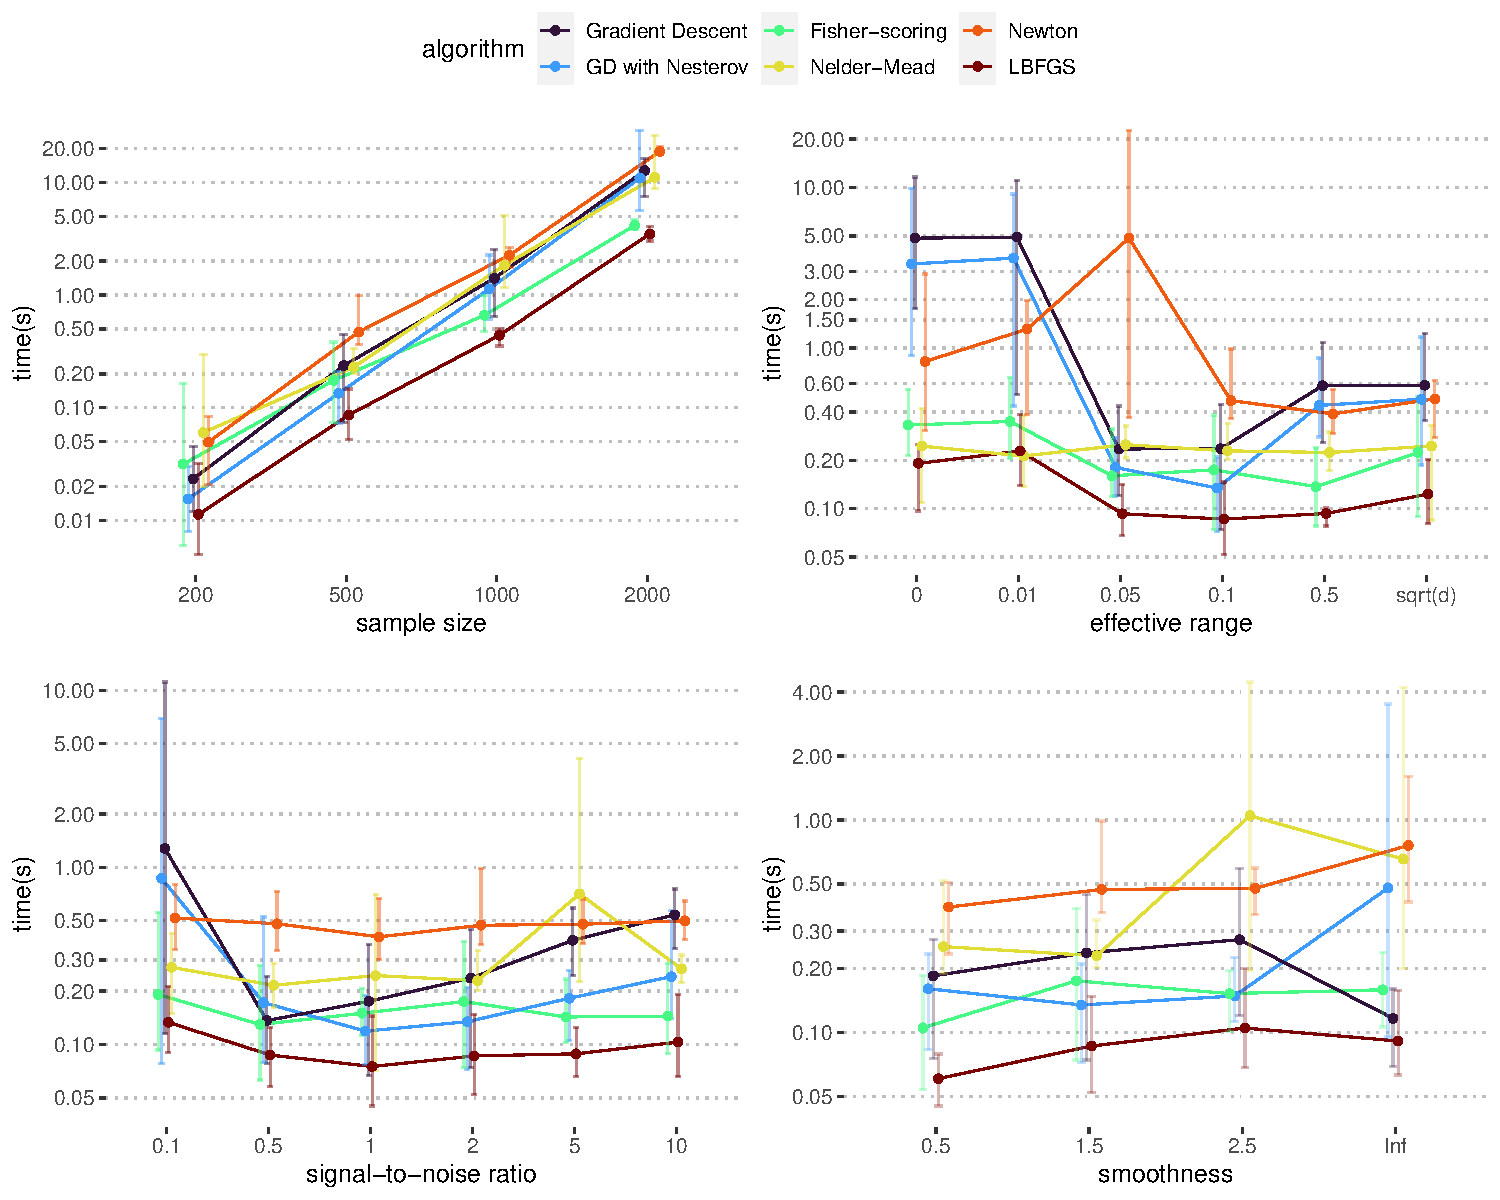
\includegraphics[width=.9\textwidth]{matern_0510} %<< no file extension
  %%         --- .5\textwidth stands for 50% of text width
  \caption[Times of simulated GP-Matern starting at default values: line graphs with range bars]%<<-- Legend for the list of figures at the beginning of you thesis
  {Comparison of optimization methods with different sample sizes and hyper-parameters $(n,\rho, \sigma^2_f/\sigma^2_n, \nu)$, all y-axes in $\log_{10}$ scale.}% legend displayed below the graph.
  \label{fig:matern_default}
\end{figure}

\begin{figure}[hbt!]%--- Picture 'H'ere, 'B'ottom or 'T'op; '!' 
  \centering
  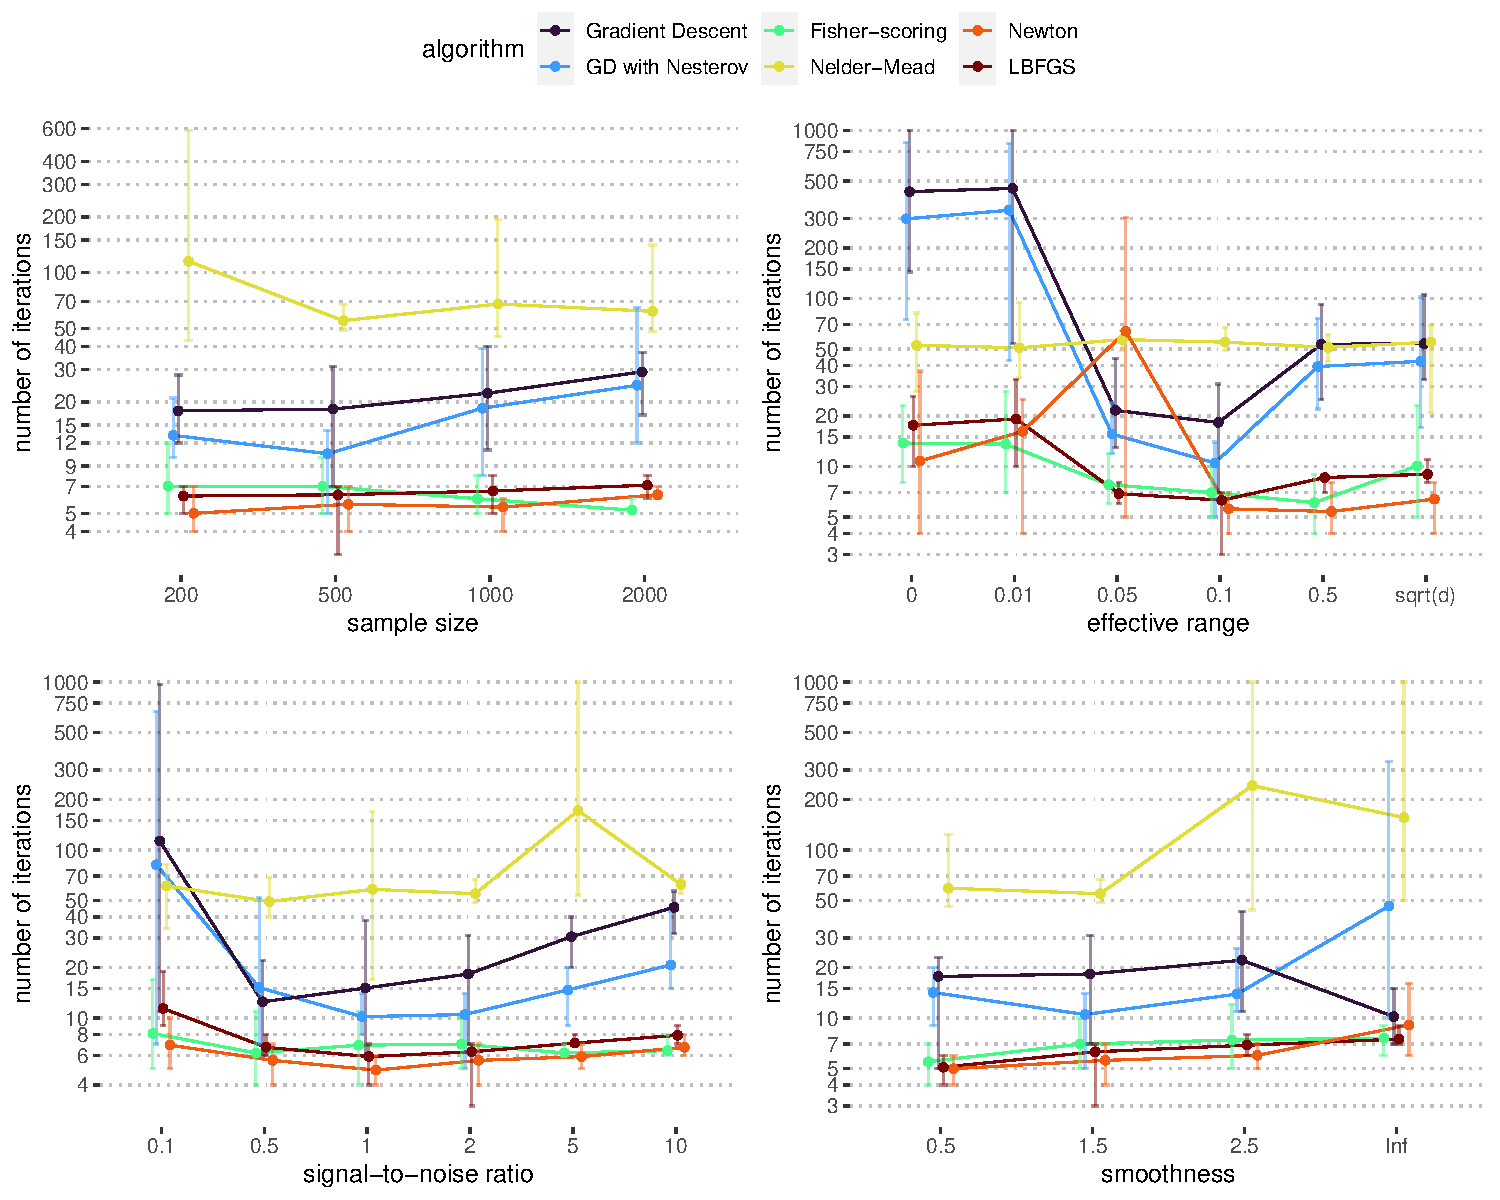
\includegraphics[width=.9\textwidth]{matern_iteration_0417} %<< no file extension
  %%         --- .5\textwidth stands for 50% of text width
  \caption[Number of iterations of simulated GP-matern starting at default values: line graphs with range bars]%<<-- Legend for the list of figures at the beginning of you thesis
  {Comparison of number of iterations of different methods, all y-axes are in $\log_{10}$ scale.}% legend displayed below the graph.
  \label{fig:matern_iteration}
\end{figure}

Figure 3.1 illustrates that LBFGS is the fastest method in most settings, and Fisher-scoring also has good performance. In most settings, Newton is the slowest method due to the need to compute the exact second derivative. 

Figure 3.2 shows that an iteration of Newton is more expensive, whereas an iteration of Nelder-Mead algorithm takes the least time. In each iteration, Newton calculates the exact second order derivative, and Nelder-Mead only evaluates the function values. Also, LBFGS, Newton, and Fisher-scoring methods mostly converge within 10 steps of iteration, and tend to require more steps in the case of small range parameter $\rho$. 

We check whether these optimization methods converge by checking the final log-likelihood values, and there are the following convergence problems:

\begin{itemize}
\item When $\rho=0$ (the simulated data is actually i.i.d Gaussian distributed), Nelder-Mead fails to converge in 2 (of 10) repetitions. 
\item When $\rho = 0.01$, Nelder-Mead fails in 3 (of 10) repetitions, Gradient Descent and GD with Nesterov accelerator both fail to converge in 2 (of 10) repetitions, Newton and LBFGS both fail in 1 (of 10) repetition.
\item When $\sigma^2_f/\sigma^2_n=0.1 \ (\sigma^2_n=10)$, Nelder-Mead fails to converge in 1 (of 10) repetition.
\item When $\sigma^2_f/\sigma^2_n=5 \ (\sigma^2_n=0.2)$, Nelder-Mead fails to converge in 1 (of 10) repetition.
\item When $\nu = 2.5$, Nelder-Mead fails to converge in 2 (of 10) repetitions.
\item When $\nu = \inf $, Nelder-Mead fails to converge in 1 (of 10) repetition.
\end{itemize}

We perform experiments with larger sample size with FITC and Vecchia approximations separately, resulting in four sets of experiment results in Figure 3.3. All repetitions of experiments result in successful convergence.

\begin{figure}[hbt!]%--- Picture 'H'ere, 'B'ottom or 'T'op; '!' 
  \centering
  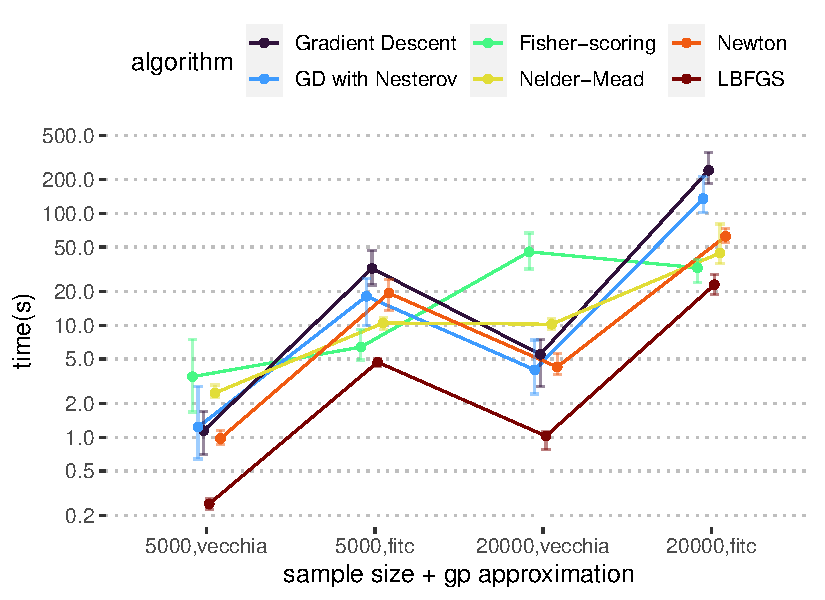
\includegraphics[width=.5\textwidth]{matern_approx_stable} %<< no file extension
  %%         --- .5\textwidth stands for 50% of text width
  \caption[Times of simulated GP-Matern using approximation: line graphs with range bars]%<<-- Legend for the list of figures at the beginning of you thesis
  {Comparison of times of different methods with approximation enabled, y-axis in $\log_{10}$ scale.}% legend displayed below the graph.
  \label{fig:matern_iteration}
\end{figure}

Figure 3.3 shows that LBFGS still outperforms the other methods with approximation enabled, and using the Vecchia approximation for GP models seems to be more efficient on average than FITC. LBFGS has the most stable performance, which can be deduced from the shorter vertical distances between bars. However, the approximate calculation of Fisher information with Vecchia in the implementation of \texttt{GPBoost} makes it slower than the other optimization methods, and in this sense, it is an unfair comparison between Fisher Scoring and other optimization methods in the presence of Vecchia approximation.

\subsubsection{Different initialization}
To investigate the influence of the starting points of the hyper-parameters on the optimization, we repeat the experiments in Figure 3.1, but with the starting values as true values and with inappropriately large values, which corresponds to the results in Figure 3.4 and Figure 3.5 respectively.

\begin{figure}[hbt!]%--- Picture 'H'ere, 'B'ottom or 'T'op; '!' Try to
                    %impose your will to LaTeX
  \centering
  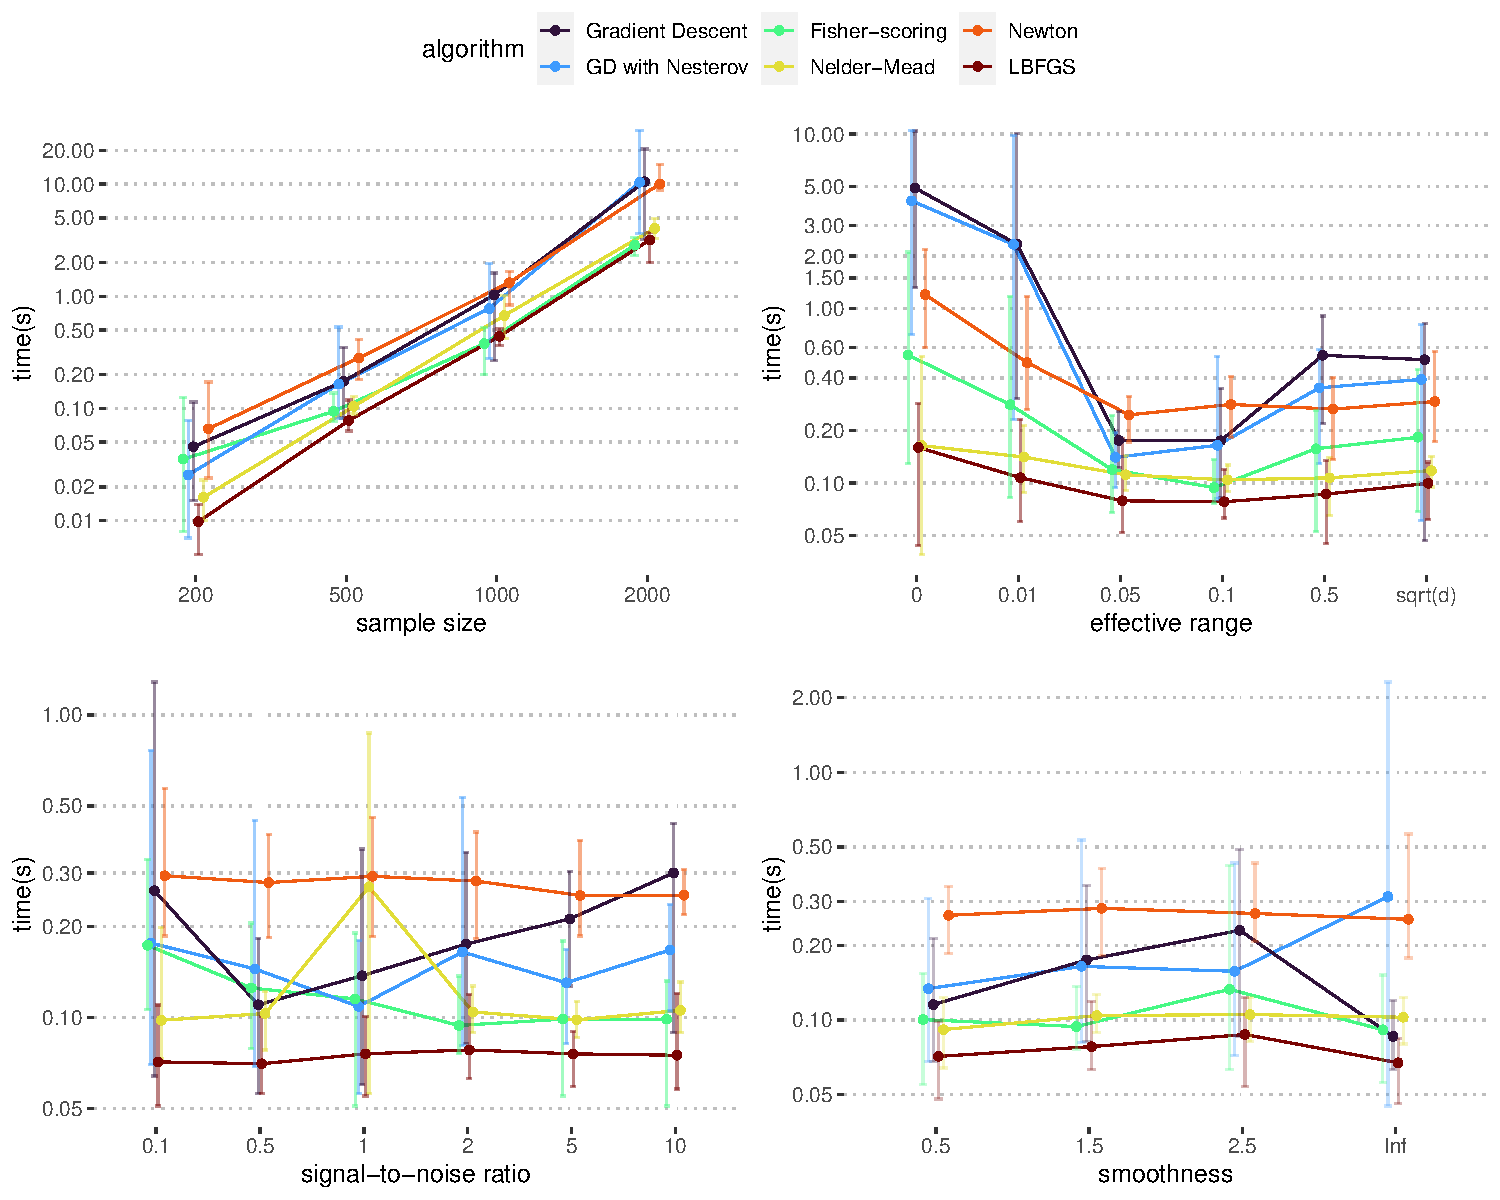
\includegraphics[width=.9\textwidth]{matern_init_true} %<< no file extension
  %%         --- .5\textwidth stands for 50% of text width
  \caption[Times of simulated GP-Matern starting at true values: line graphs with range bars]%<<-- Legend for the list of figures at the beginning of you thesis
  {Comparison of different optimization methods with different sample sizes and hyper-parameters, starting at true values, all y-axes in $\log_{10}$ scale.}
  \label{fig:matern_init_true}
\end{figure}

\begin{figure}[hbt!]%--- Picture 'H'ere, 'B'ottom or 'T'op; '!' Try to
                    %impose your will to LaTeX
  \centering
  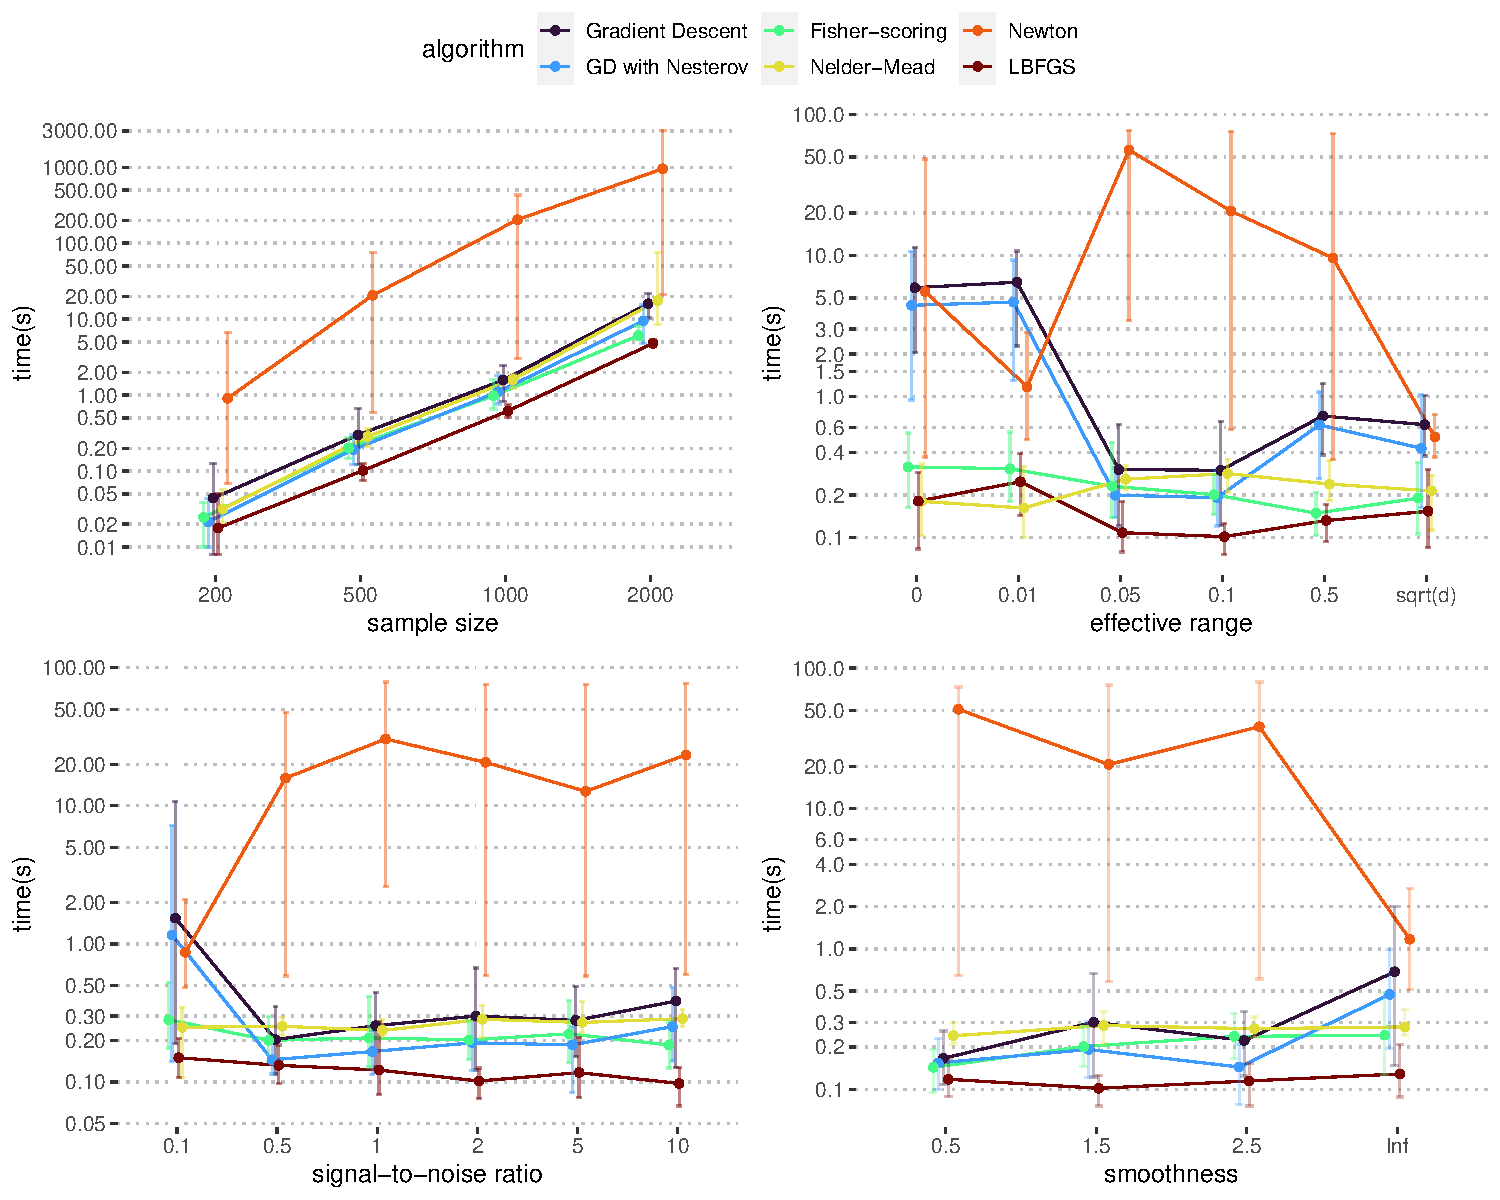
\includegraphics[width=.9\textwidth]{matern_init_unreas} %<< no file extension
  %%         --- .5\textwidth stands for 50% of text width
  \caption[Times of simulated GP-Matern starting at large values: line graphs with range bars]%<<-- Legend for the list of figures at the beginning of you thesis
  {Comparison of different algorithms with different sample sizes and hyper-parameters, starting at large values, 10 repetitions. All y-axes are in $\log 10$ scale.}% legend displayed below the graph.
  \label{fig:matern_init_unreas}
\end{figure}

Comparing Figures 3.4 and 3.5 with Figure 3.1, we can conclude that LBFGS is the fastest method in most experiments with any initialization strategy. Newton is sensitive to the choice of starting point, reflected by the phenomenon that starting from points far from the optima makes it difficult to converge within the iteration limit. However, if a suitable starting point is chosen, Fisher-scoring or Nelder-Mead can be as fast as LBFGS.

When starting the iteration from true values, all optimization methods successfully converge to the optima and consume less time compared to the other two initialization strategies. It is intuitive that the time of any optimizer will be longer if it starts iterating from an unreasonably distant point instead of a reasonable point related to the sample. Also, the convergence problem with unreasonable starting points in Figure 3.5 is more severe than with the default initialization:

\begin{itemize}
%\item Newton is manually excluded from experiments of $n=20000$ as it is extremely slow.
\item In the default setting ($n=500, \rho=0.1, \sigma^2_f/\sigma^2_n = 2$, and $\nu=1.5$), Newton fails to converge in 2 (of 10) repetitions.
\item When $n=1000$, Newton fails to converge in 4 (of 10) repetitions.
\item When $n=2000$, Newton fails to converge in 3 (of 10) repetitions.
%\item When $n=5000$, Newton fails in 8 (of 10) repetitions, Fisher-scoring fails to converge in 4 (of 10) repetitions.
\item When $\rho=0$, Nelder-Mead and LBFGS fails both in 1 (of 10) repetition.
\item When $\rho=0.01$, GD, GD with Nesterov accelerator and LBFGS all fails in 1 (of 10) repetition.
\item When $\rho=0.05$, Newton fails to converge in 7 (of 10) repetitions.
\item When $\rho=0.5$, Newton fails to converge in 1 (of 10) repetition.
\item When $\sigma^2_f/\sigma^2_n = 0.1$, Nelder-Mead and Newton both fail in 2 (of 10) repetitions.
\item When $\sigma^2_f/\sigma^2_n = 1$, Newton fails to converge in 2 (of 10) repetitions.
\item When $\sigma^2_f/\sigma^2_n = 5$, Newton fails to converge in 1 (of 10) repetition.
\item When $\sigma^2_f/\sigma^2_n = 5$, Newton fails to converge in 3 (of 10) repetitions.
\item When $\nu=0.5$, Newton fails in 5 (of 10) repetitions.
\item When $\nu=2.5$, Newton fails in 5 (of 10) repetitions.
\end{itemize}

\subsubsection{BFGS-based methods}

Considering the good performance of LBFGS, we further compare five variants of BFGS methods available in R. Two approximations are still enabled for large data. Besides ``lbfgs" in \texttt{GPBoost}, which we have experimented with, we also introduce ``lbfgs\_not\_profile \_out\_nugget" from \texttt{GPBoost}, and BFGS, L-BFGS-B and L-BFGS (L-BFGS-B with no bound on hyper-parameters) from \texttt{optim} function. 

The results are displayed in Figures 3.6 and 3.7, which show that ``lbfgs" is faster than ``lbfgs\_not\_profile\_out\_nugget", and they both significantly beat the three optimization methods in \texttt{optim}. In addition, some methods have convergence problems:

\begin{itemize}
    \item When $\rho=0$, L-BFGS-B(optim) fails to converge in 1 (of 10) repetition.
    \item When $\rho=0.01$, L-BFGS-B(optim) fails to converge in 3 (of 10) repetitions, ``lbfgs\_not\_profile\_out\_nugget" fails to converge in 2 (of 10) repetitions.
    \item When $\rho=\sqrt{2}$, BFGS(optim) fails to converge in 1 (of 10) repetition.
    \item When $\sigma^2_f/\sigma^2_n = 0.1$, L-BFGS-B(optim) fails to converge in 2 (of 10) repetitions.
    \item When $n=20000$ and using FITC approximation, BFGS(optim) fails to converge in 2 (of 10) repetitions.
\end{itemize}

\begin{figure}[hbt!]%--- Picture 'H'ere, 'B'ottom or 'T'op; '!' Try to
                    %impose your will to LaTeX
  \centering
  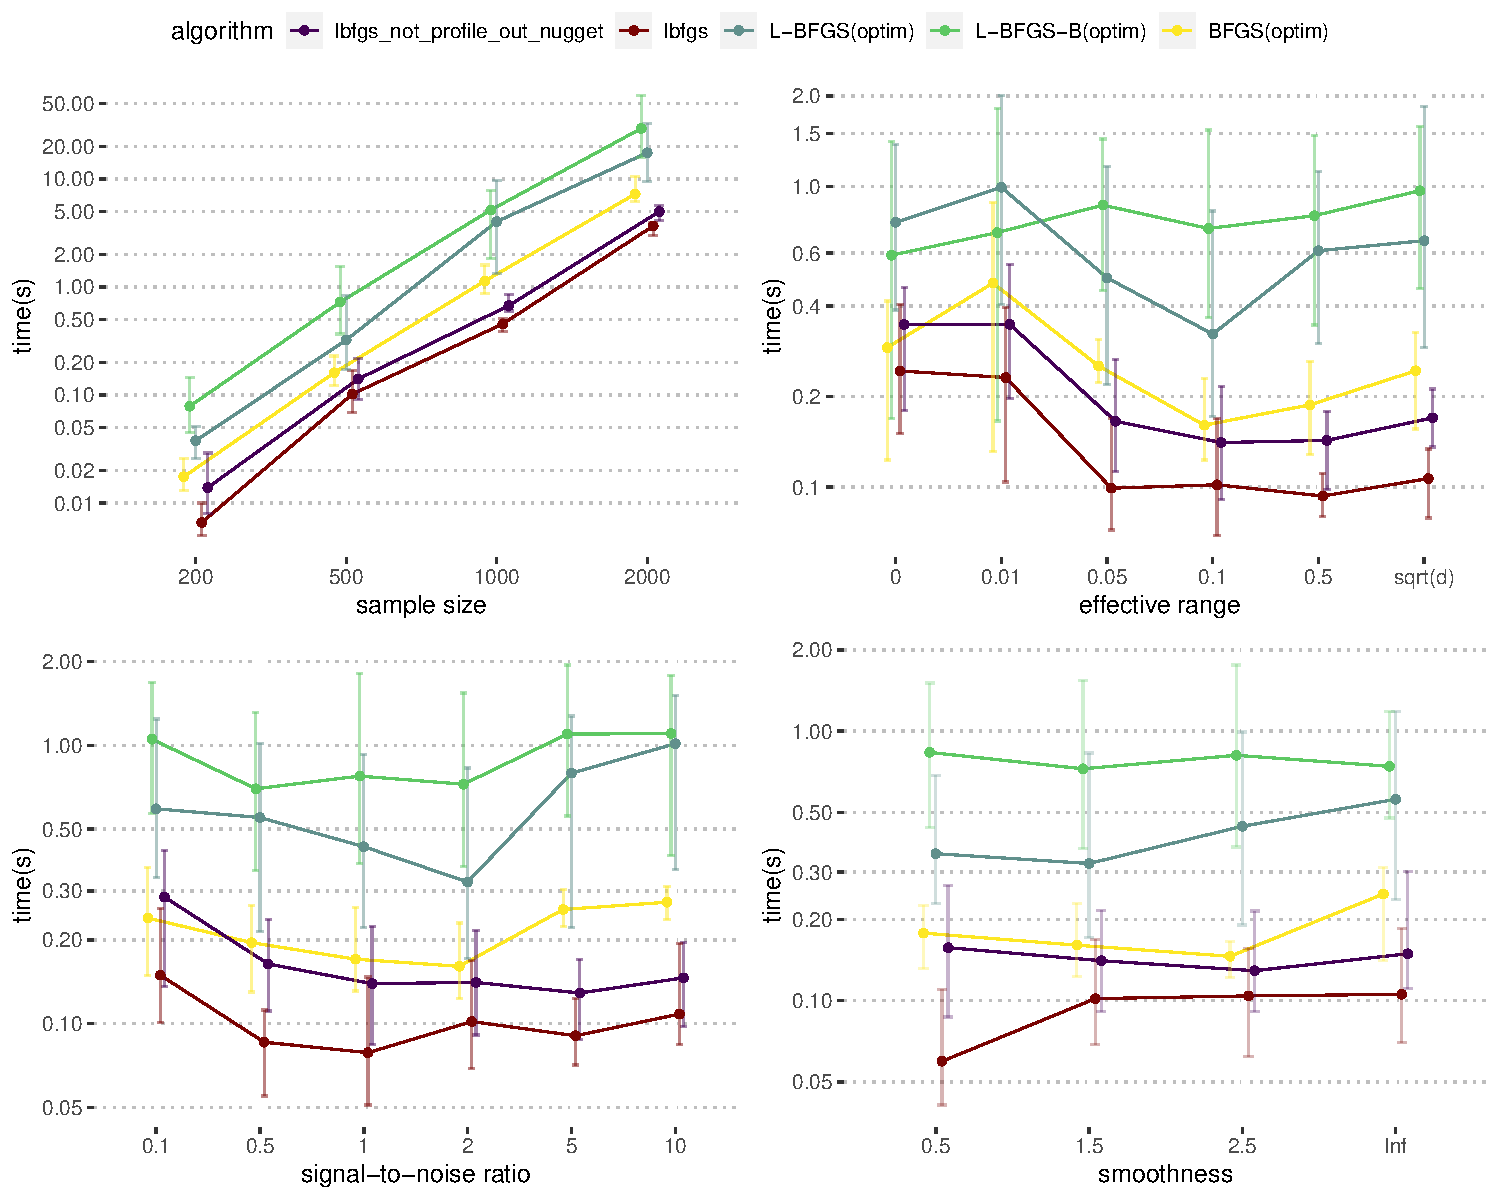
\includegraphics[width=.9\textwidth]{matern_bfgs_0606} %<< no file extension
  %%         --- .5\textwidth stands for 50% of text width
  \caption[Comparison of BFGS variants: times of GP-Matern starting at default values: line graphs with range bars]%<<-- Legend for the list of figures at the beginning of you thesis
  {Comparison of BFGS-based algorithms with different sample sizes and hyper-parameters, starting at default values, all Y-axes are in $\log_{10}$ scale.}% legend displayed below the graph.
  \label{fig:matern_bfgs}
\end{figure}

\begin{figure}[hbt!]%--- Picture 'H'ere, 'B'ottom or 'T'op; '!' 
  \centering
  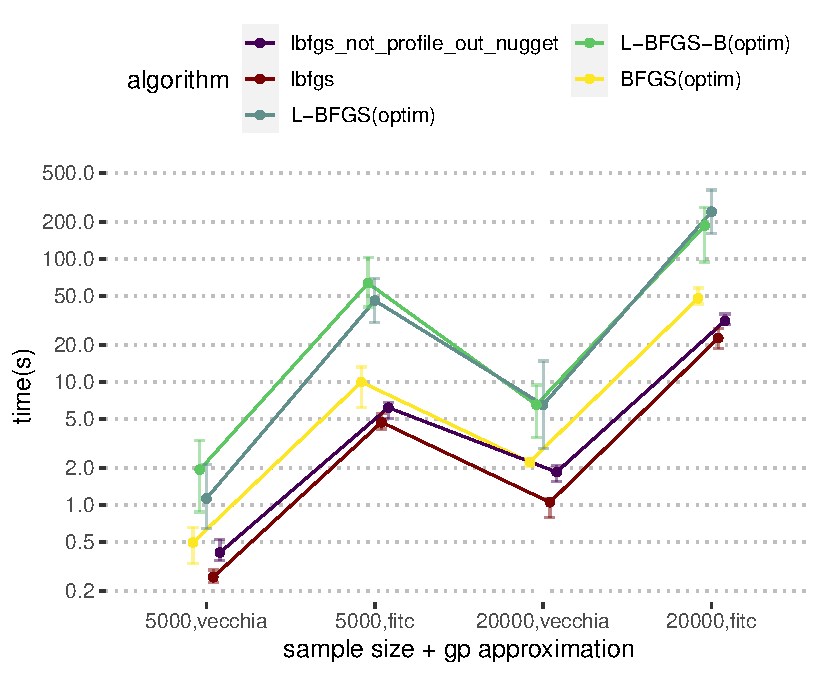
\includegraphics[width=.5\textwidth]{bfgs_approx_stable} %<< no file extension
  %%         --- .5\textwidth stands for 50% of text width
  \caption[Comparison of BFGS variants with approximation: times of GP-Matern starting at default values: line graphs with range bars]%<<-- Legend for the list of figures at the beginning of you thesis
  {Comparison of times of BFGS methods with approximation on zero-mean GP models, y-axis in $\log_{10}$ scale.}% legend displayed below the graph.
  \label{fig:linear_iteration}
\end{figure}


\subsection{GP with Non-zero mean}

To further investigate the performance of the optimization methods on GP models, we add the linear regression term $\boldsymbol{Z\beta}$ as the mean function $m(\bold{x})$:

\begin{equation}
    \pmb{z} = [1, z_{1},...,z_{9}], \ \boldsymbol{\beta} = [0,1,...,1] \text{, where } z_{i}\overset{\mathrm{iid}}{\sim} N(0, 0.1).
\end{equation}

Now we need to estimate the hyper-parameters $(\rho, \sigma^2_f, \sigma^2_n)$ and the linear coefficients $\boldsymbol{\beta}$. The experimental settings of hyper-parameters in section 3.1.1 are applied again. The experimental results are shown in Figure 3.8, and the large scale optimization results are shown in Figure 3.9. Note that Nelder-Mead method is excluded because it is unable to converge to the optima in any setting, and it takes a long time to search in each step. The heuristic search strategy of Nelder-Mead makes it difficult to solve the problem when the number of parameters to be estimated increases enormously. 

\begin{figure}[hbt!]%--- Picture 'H'ere, 'B'ottom or 'T'op; '!' Try to
                    %impose your will to LaTeX
  \centering
  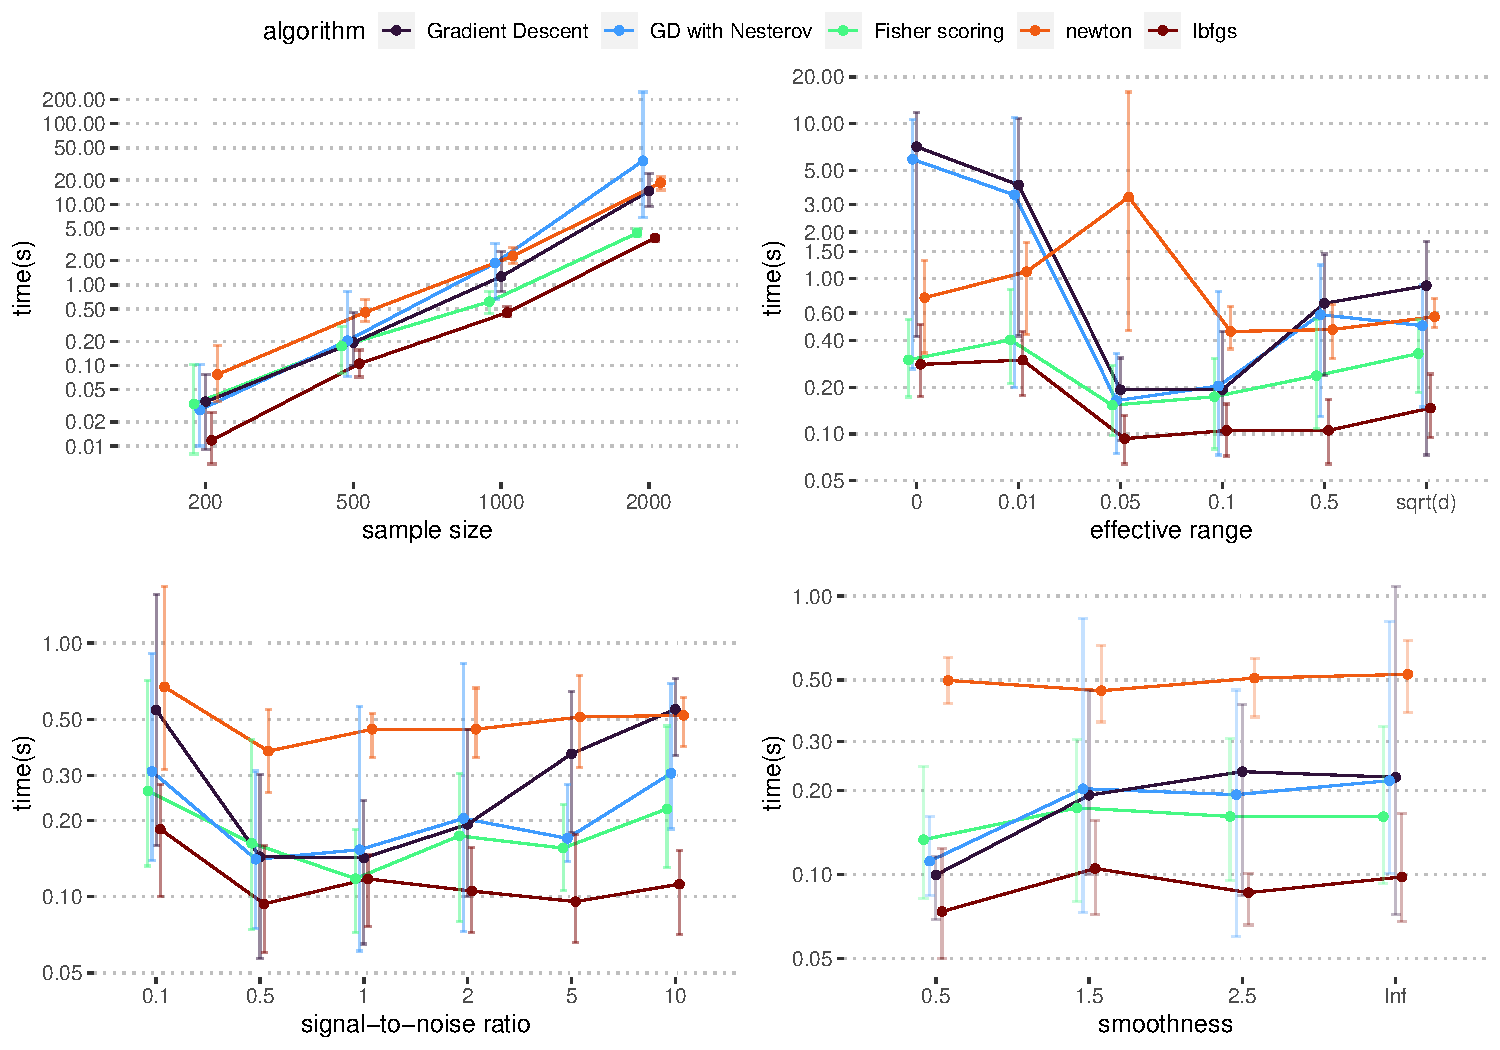
\includegraphics[width=.9\textwidth]{matern_linear_reg} %<< no file extension
  %%         --- .5\textwidth stands for 50% of text width
  \caption[Times of GP-Matern with linear regression terms: line graphs with range bars]%<<-- Legend for the list of figures at the beginning of you thesis
  {Comparison of different methods of GP models with added linear regression term, default starting values, all y-axes are in $\log_{10}$ scale.}
  \label{fig:matern_linear}
\end{figure}

Compared to the results of the zero-mean GP models in Figure 3.1, Figure 3.8 shows that the relative ranking among the optimization methods and the average time used by each method remain the same after introducing the linear regression term, and LBFGS still has outstanding performance. Results in Figure 3.9 show that LBFGS and Newton take the least time in large scale optimization.

The convergence check shows that:
\begin{itemize}
    \item When $\rho=0.01$, GD, GD with Nesterov accelerator and Newton all fail to converge in 1 (of 10) repetition.
    \item When $n=5000$ and using Vecchia approximation, Newton's method fails to converge in 1 (of 10) repetition.
\end{itemize}

\begin{figure}[hbt!]%--- Picture 'H'ere, 'B'ottom or 'T'op; '!' 
  \centering
  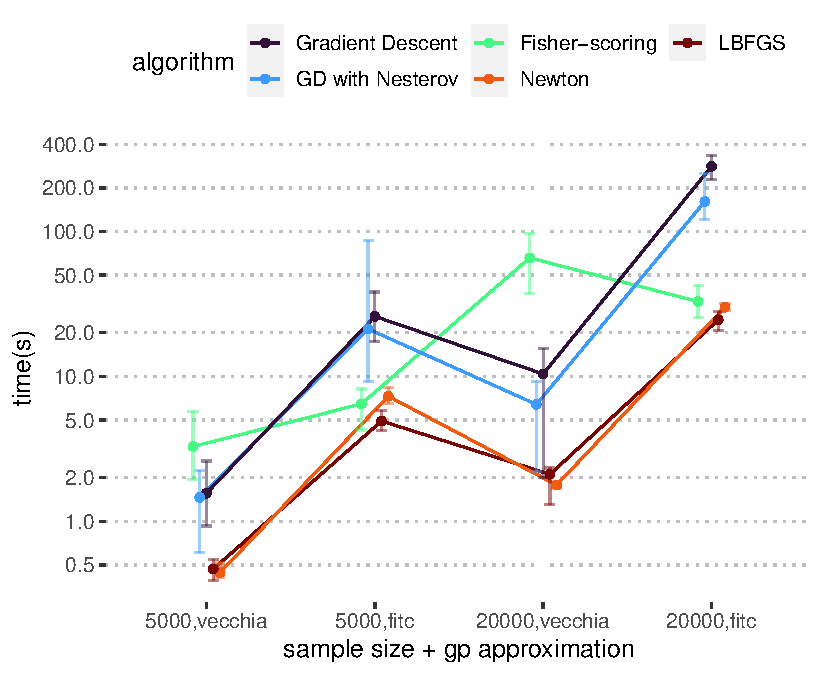
\includegraphics[width=.5\textwidth]{linear_approx_stable} %<< no file extension
  %%         --- .5\textwidth stands for 50% of text width
  \caption[Times of GP-Matern with linear regression term using approximation: line graphs with range bars]%<<-- Legend for the list of figures at the beginning of you thesis
  {Comparison of times of different methods with approximation on model with linear terms, y-axis in $\log_{10}$ scale.}% legend displayed below the graph.
  \label{fig:linear_iteration}
\end{figure}

\subsection{Binary data}

The observation variables are categorical in some applications, where GP classification models are applied. Therefore, we test the performance of optimization methods on GP models with binary likelihood (Bernoulli distribution with \textit{logit} link function). In this section, similar settings of hyper-parameters are used, whereas the noise term is no longer included in the data simulation. Instead of the signal-to-noise ratio, we only change the signal variance in the experiment. The results are displayed in Figurea 3.10 and 3.11, note that Fisher-scoring is excluded in the results, because the Fisher information is not computable for GP with binary likelihood. The convergence check shows that, when $n=5000$ and using FITC approximation, Newton fails to converge in 1 (of 10) repetition.

\begin{figure}[hbt!]%--- Picture 'H'ere, 'B'ottom or 'T'op; '!' Try to
                    %impose your will to LaTeX
  \centering
  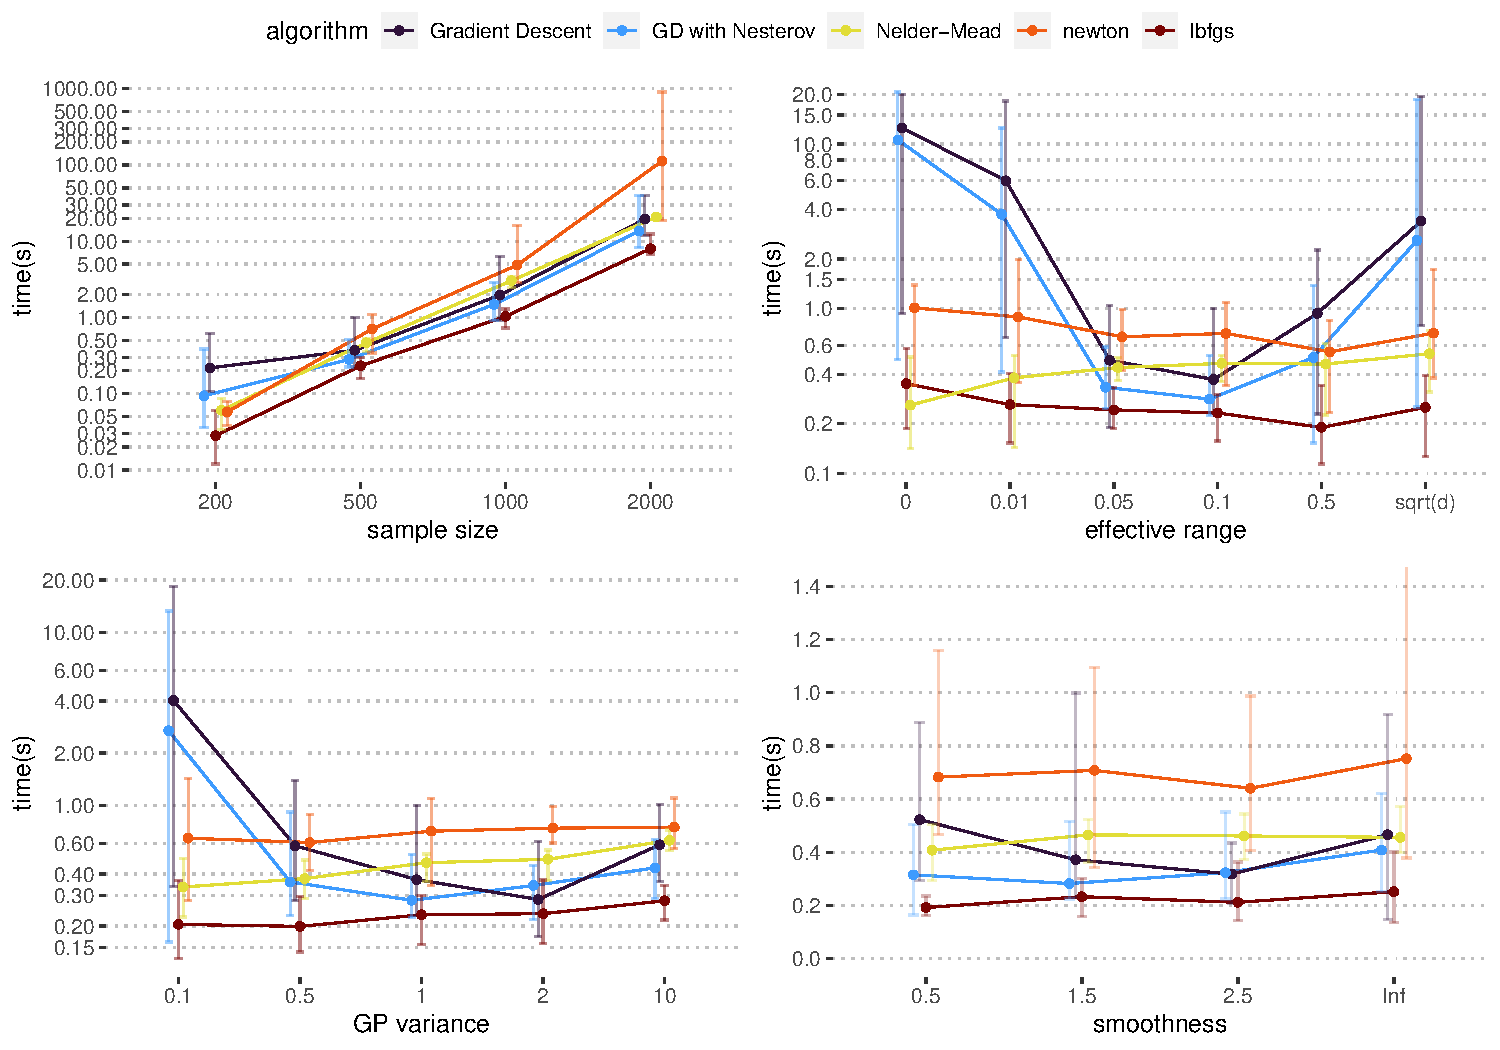
\includegraphics[width=.9\textwidth]{matern_binary_0426} %<< no file extension
  %%         --- .5\textwidth stands for 50% of text width
  \caption[Times of GP-Matern with Binary likelihood: line graphs with range bars]%<<-- Legend for the list of figures at the beginning of you thesis
  {Comparison of methods on GP with binary likelihood of different sample sizes and hyper-parameters, all y-axes except lower-right sub-figure are in $\log_{10}$ scale.}% legend displayed below the graph.
  \label{fig:matern_binary}
\end{figure}

\begin{figure}[hbt!]%--- Picture 'H'ere, 'B'ottom or 'T'op; '!' 
  \centering
  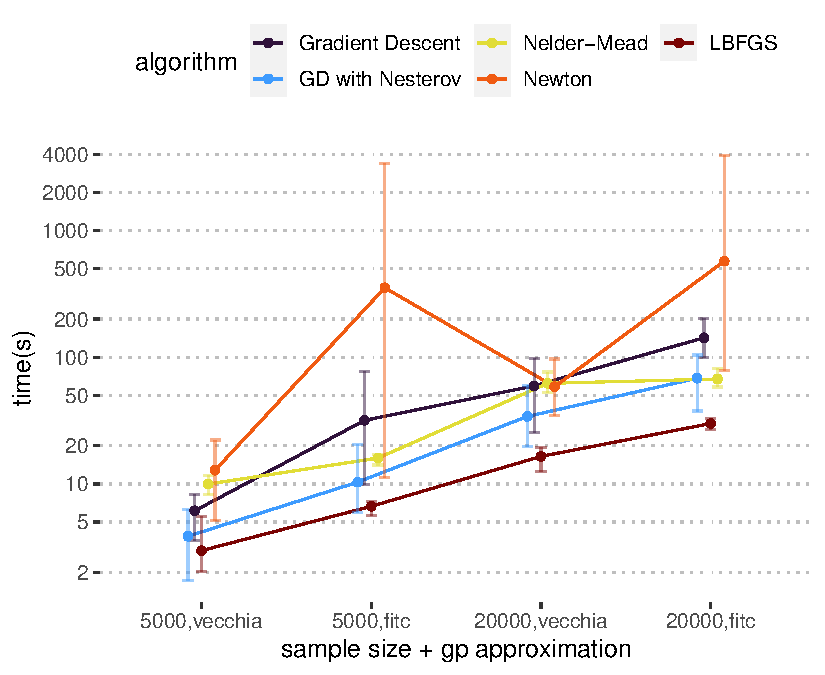
\includegraphics[width=.5\textwidth]{binary_approx_stable} %<< no file extension
  %%         --- .5\textwidth stands for 50% of text width
  \caption[Times of  GP-Matern with binary likelihood using approximation: line graphs with range bars]%<<-- Legend for the list of figures at the beginning of you thesis
  {Comparison of times of different methods with approximation on model with binary likelihood, y-axis in $\log_{10}$ scale.}% legend displayed below the graph.
  \label{fig:linear_iteration}
\end{figure}

Furthermore, we again add the linear regression terms as in Eq.(5) into the GP classification models. The performance comparison of four algorithms (GD, GD with Nesterov accelerator, Nelder Mead, and LBFGS) is displayed in Figure 3.12 and Figure 3.13. In these experiments, Newton's method faces some convergence problems:

\begin{itemize}
    \item When $\rho=0.01$, Newton fails to converge in 1 (of 10) repetition.
    \item When $\sqrt d$, Newton fails to converge in 1 (of 10) repetition.
    \item When n=20000 and using FITC approximation, Newton fails to converge in 2 (of 10) repetitions.
\end{itemize}

\begin{figure}[hbt!]%--- Picture 'H'ere, 'B'ottom or 'T'op; '!' Try to
                    %impose your will to LaTeX
  \centering
  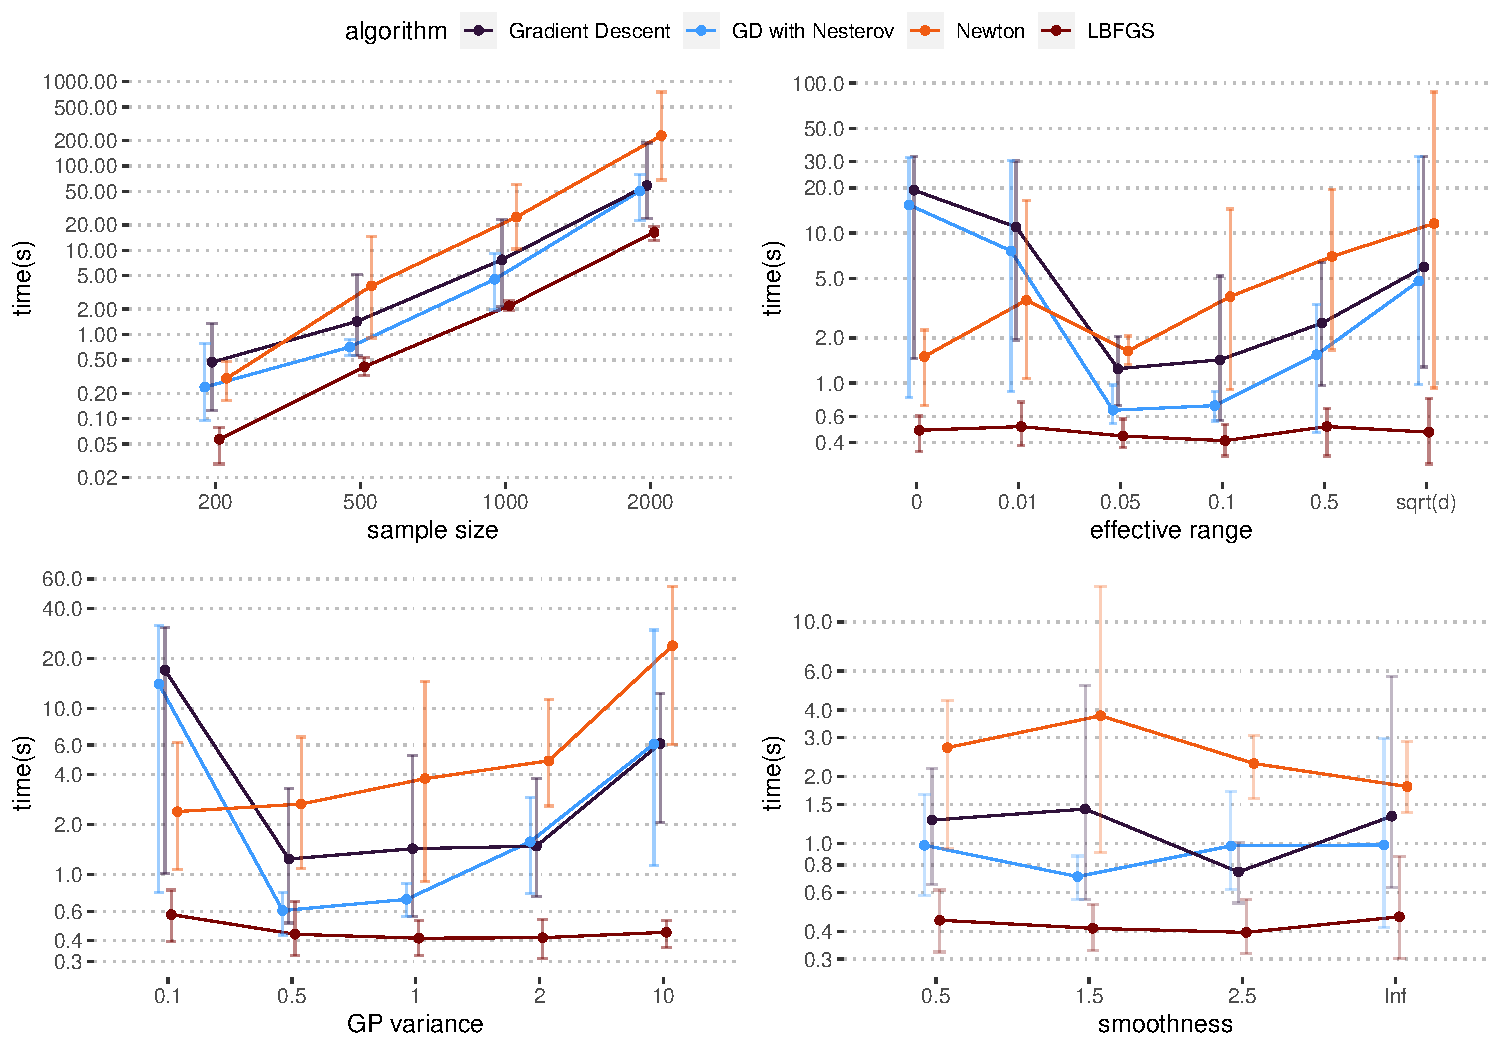
\includegraphics[width=.9\textwidth]{binary_linear_0426} %<< no file extension
  %%         --- .5\textwidth stands for 50% of text width
  \caption[Times of GP-Matern with Binary likelihood and linear regression terms: line graphs with range bars]%<<-- Legend for the list of figures at the beginning of you thesis
  {Comparison of different methods on GP with binary likelihood and added linear regression terms, all y-axes are in $\log_{10}$ scale.}% legend displayed below the graph.
  \label{fig:binary_linear}
\end{figure}

\begin{figure}[hbt!]%--- Picture 'H'ere, 'B'ottom or 'T'op; '!' 
  \centering
  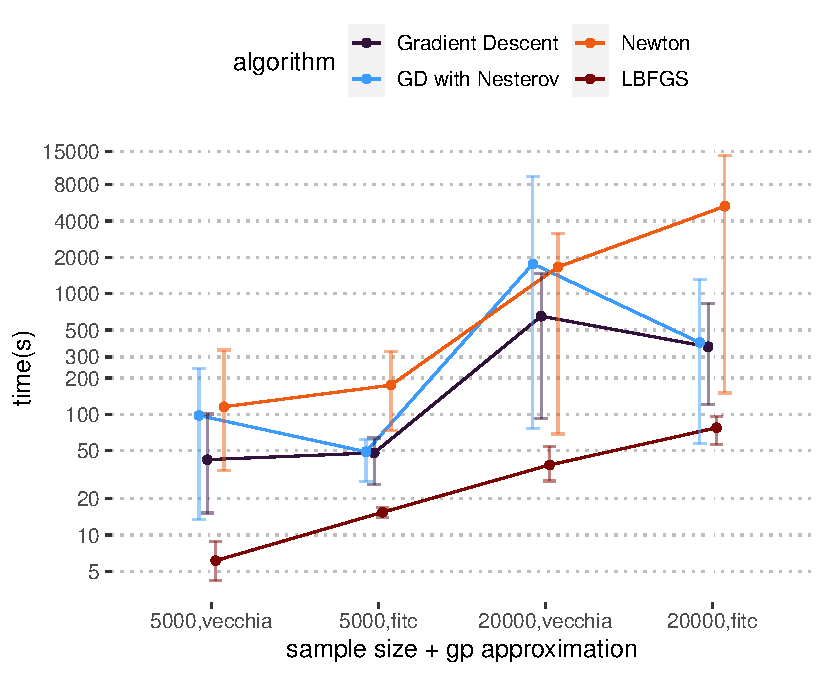
\includegraphics[width=.5\textwidth]{binary_linear_approx_stable} %<< no file extension
  %%         --- .5\textwidth stands for 50% of text width
  \caption[Times of GP-Matern with binary likelihood and linear regression terms using approximation: line graphs with range bars]%<<-- Legend for the list of figures at the beginning of you thesis
  {Comparison of times of different methods with approximation on model with binary likelihood and linear regression terms, y-axis in $\log_{10}$ scale.}% legend displayed below the graph.
  \label{fig:linear_iteration}
\end{figure}

From Figures 3.10, 3.11, 3.12 and 3.13 in this section, similar conclusions can be drawn; LBFGS is still excellent, followed by Nelder-Mead method and two GD methods, and Newton's method is the slowest one in most cases and shows instability, which is reflected by the large gap between maximum and minimum times. Gradient Descent methods are limited by the long-ridge and flat likelihood, which is illustrated by the slower optimization in the models with small range.

\section{Mis-specified models}

In Section 3.1, we have performed several experiments based on the GP models with Mat\'ern class covariance function, when we have used correctly specified models in the model fitting stage. In this section, performance of optimization methods in the situation of model mis-specification will be compared, which means that the GP model used for fitting belongs to a different distribution class than the model used for data simulation. In our experiments, the data sample is simulated from GP with Mat'ern covariance function with smoothness $\nu = 0.5/ \inf$, and then optimized using the GP model with different smoothness value.

Again, we consider the application of a smaller sample and a large sample of size 5000 (using Vecchia and FITC) and fit a GP model with different smoothness values. The results of data simulated by GP models with smoothness $\nu=0.5$ (exponential covariance) are shown in Figure 3.14. Figure 3.15 displays the results of smoothness $\nu \xrightarrow{} \infty$ (squared exponential or Gaussian covariance). The figures are divided into two parts: left for the experiments with smaller sample size, right for the large sample with Vecchia and FITC approximation.

\begin{figure}[hbt!]%--- Picture 'H'ere, 'B'ottom or 'T'op; '!' Try to
                    %impose your will to LaTeX
  \centering
  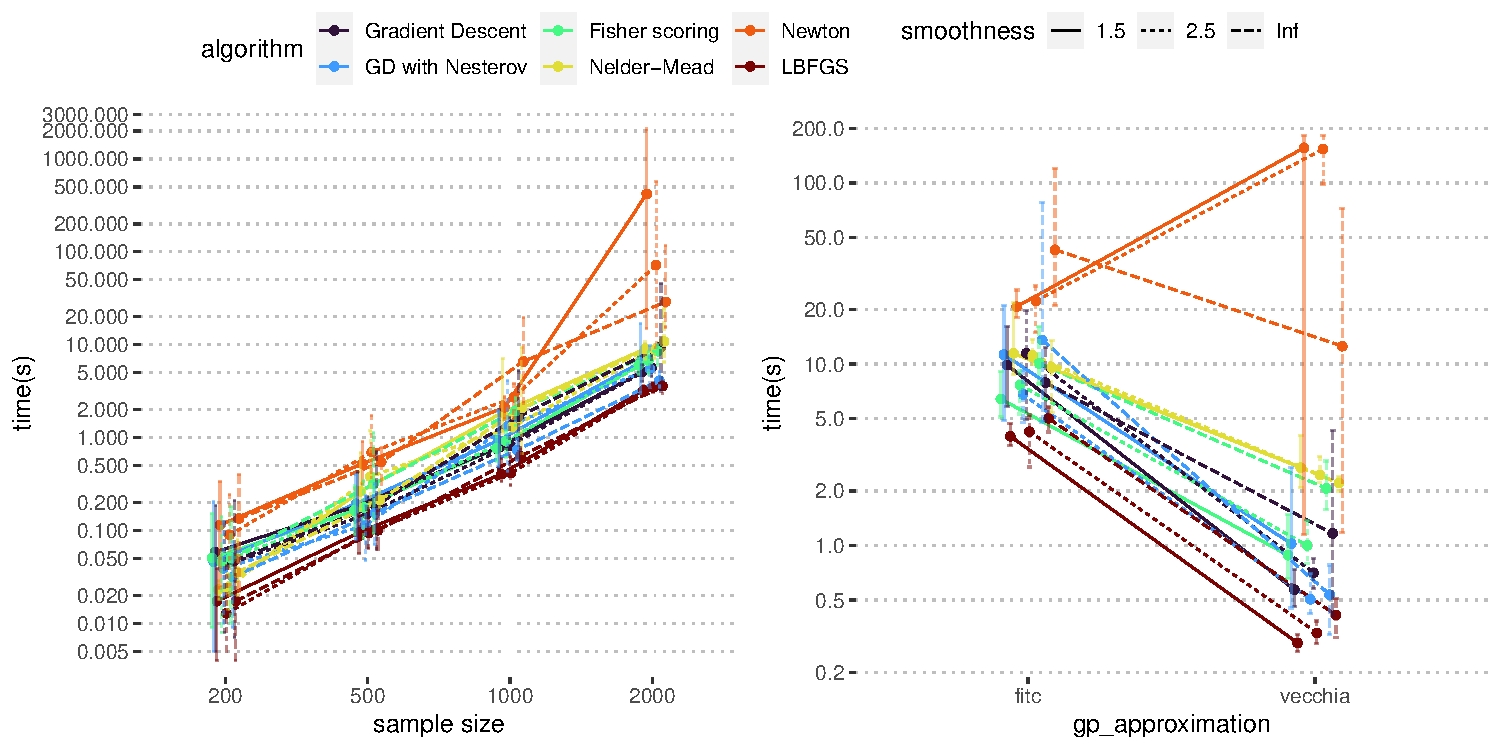
\includegraphics[width=.9\textwidth]{misspec_0.5_stable} %<< no file extension
  %%         --- .5\textwidth stands for 50% of text width
  \caption[Times of mis-specified GP with 0.5 smoothness: graphs of different line types with range bars]%<<-- Legend for the list of figures at the beginning of you thesis
  {Comparison of different methods using mis-specified GP models on data from GP with 0.5 smoothness, default starting values, 10 repetitions. Y-axis is in $\log 10$ scale. Vecchia approximation is utilized when n = 5000}% legend displayed below the graph.
  \label{fig:matern_mis_0.5}
\end{figure}

Figure 3.14 shows that LBFGS has the best performance with any smoothness parameters, and Newton is the slowest. The convergence check of this figure shows that for large data of 5000 points:

\begin{itemize}
    \item When $\nu=1.5$ and using Vecchia approximation, Newton fails to converge in 7 (of 10) repetitions.
    \item When $\nu=2.5$ and using Vecchia approximation, Newton fails to converge in 5 (of 10) repetitions.
\end{itemize} 

\begin{figure}[hbt!]%--- Picture 'H'ere, 'B'ottom or 'T'op; '!' Try to
                    %impose your will to LaTeX
  \centering
  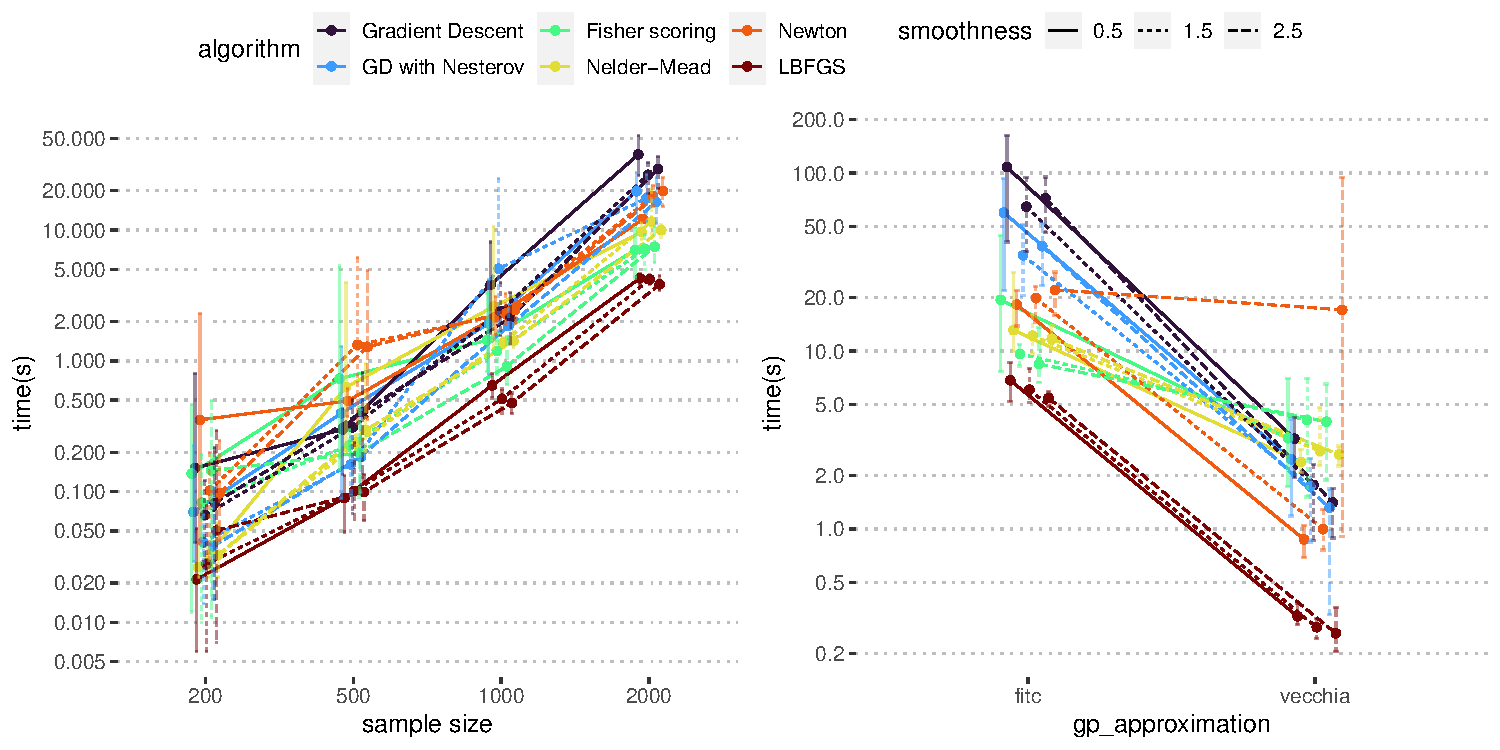
\includegraphics[width=.9\textwidth]{misspec_inf_stable} %<< no file extension
  %%         --- .5\textwidth stands for 50% of text width
  \caption[Times of mis-specified GP with infinite smoothness: graphs of different line types with range bars]
  {Comparison of different methods using mis-specified GP models on data from GP with infinite smoothness, default starting values, 10 repetitions. Y-axis is in $\log 10$ scale. Vecchia approximation is utilized when n = 5000.}
  \label{fig:matern_mis_Inf}
\end{figure}

bFor experiments of data from GP model of Gaussian covariance (infinite smoothness value), the convergence check shows that:

\begin{itemize}
    \item When $\nu=0.5, n=200$, Newton fails to converge in 6 (of 10) repetitions.
    \item When $\nu=0.5, n=500$, Nelder-Mead fails to converge in 1 (of 10) repetition.
\end{itemize} 
 
\section{Deterministic functions}

In this section, we introduce three deterministic functions for simulation experiments: Branin, Borehole and Piston (\cite{simulationlib}), and compare the performance of the optimization methods. We sample data from the functions and estimate the hyper-parameters of the Mat\'ern covariance function. This is the case when not enough information is known about the underlying function and the fitting model does not belong to the same distribution family as the true model. Note that in all deterministic experiments, the data is centered first in the pre-processing. We will first experiment with data of size 1000, and in section 3.3.4 we will use the Vecchia approximation for experiments on large data of size 20000.

\subsection{Branin function}
Branin function is a 2-dimensional function that usually evaluated over the domain $[-5,10]\times[0,15]$. It is defined as:

\begin{equation}
    f(\pmb{x}) = a(x_2 - bx_1^2 + cx_1 - r)^2 + s(1 - t) \cos{x_1} + s
\end{equation}
and we take the recommended value as $a = 1, b = 5.1/4\pi^2, c = 5/\pi, r = 6, s = 10$, and $t = 1/8\pi$ from \cite{simulationlib}.

Experiment results in Figure 3.16 illustrate that, even with Nesterov accelerator, Gradient Descent algorithm needs significantly more time to converge, especially when smoothness is 1.5 or 2.5. LBFGS remains the fastest in all cases. The convergence check of Branin experiment shows that, when $\nu\xrightarrow{} \infty$, Newton's method fails to converge in 3 (of 10) repetitions.

\begin{figure}[hbt!]%--- Picture 'H'ere, 'B'ottom or 'T'op; '!' Try to
                    %impose your will to LaTeX
  \centering
  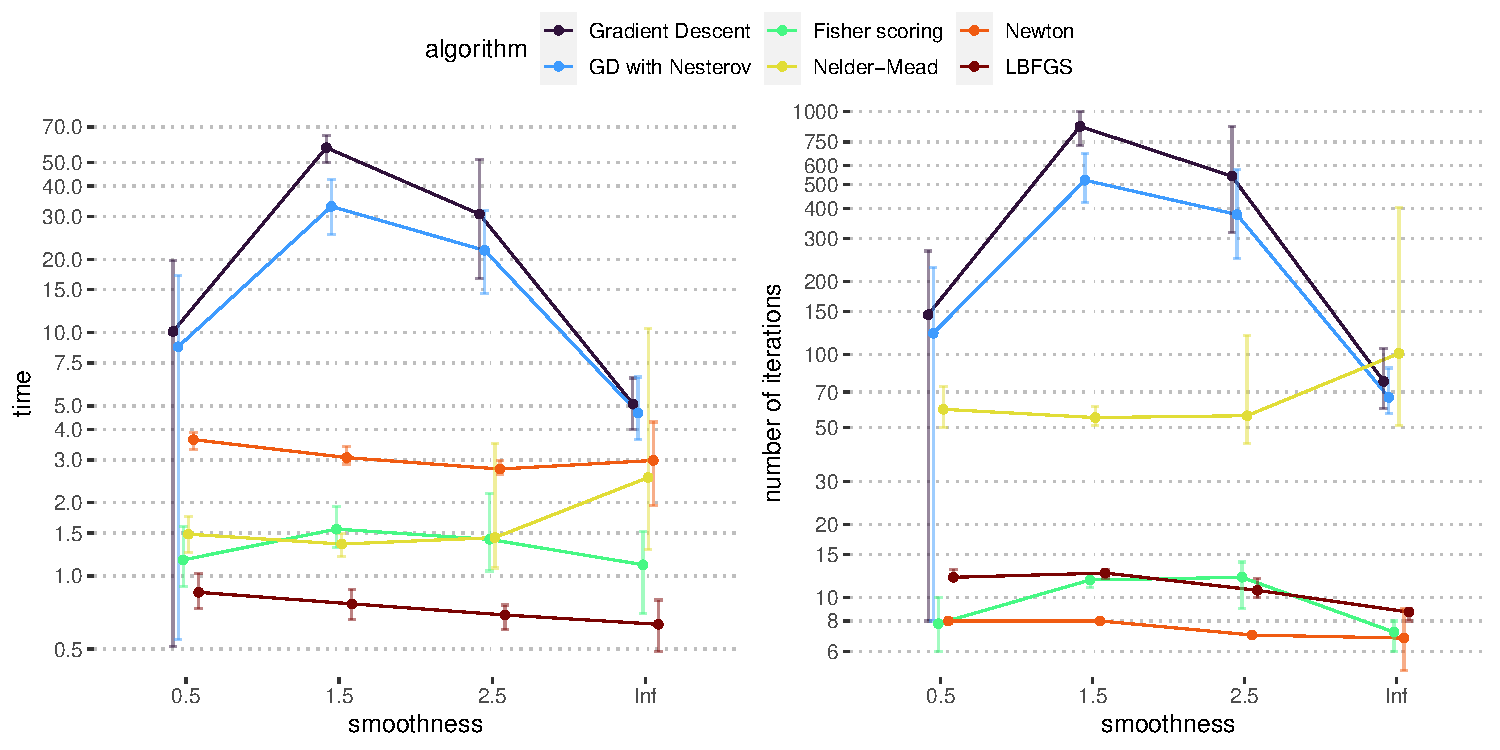
\includegraphics[width=.9\textwidth]{Branin_comparison_0426} %<< no file extension
  %%         --- .5\textwidth stands for 50% of text width
  \caption[Times of Branin function: line graphs with range bars]%<<-- Legend for the list of figures at the beginning of you thesis
  {Comparison of different methods using mis-specified GP models on data from Branin function, default starting values, 10 repetitions. Y-axes are in $\log 10$ scale.}% legend displayed below the graph.
  \label{fig:plotset}
\end{figure}

\subsection{Borehole function}
Borehole function models the flow of water through a borehole and it consists of eight input variables. Similar conclusions could be drawn from the results in Figure 3.17, except that Newton's method takes the longest average time with a large range when smoothness is 0.5. 

The convergence check shows that, when $\nu=0.5$, Newton algorithm fails to converge in 2 (of 10) repetitions. In these cases, Newton's method fails to find the optima within the prescribed of 1000 iterations limit.

\begin{figure}[hbt!]%--- Picture 'H'ere, 'B'ottom or 'T'op; '!' 
  \centering
  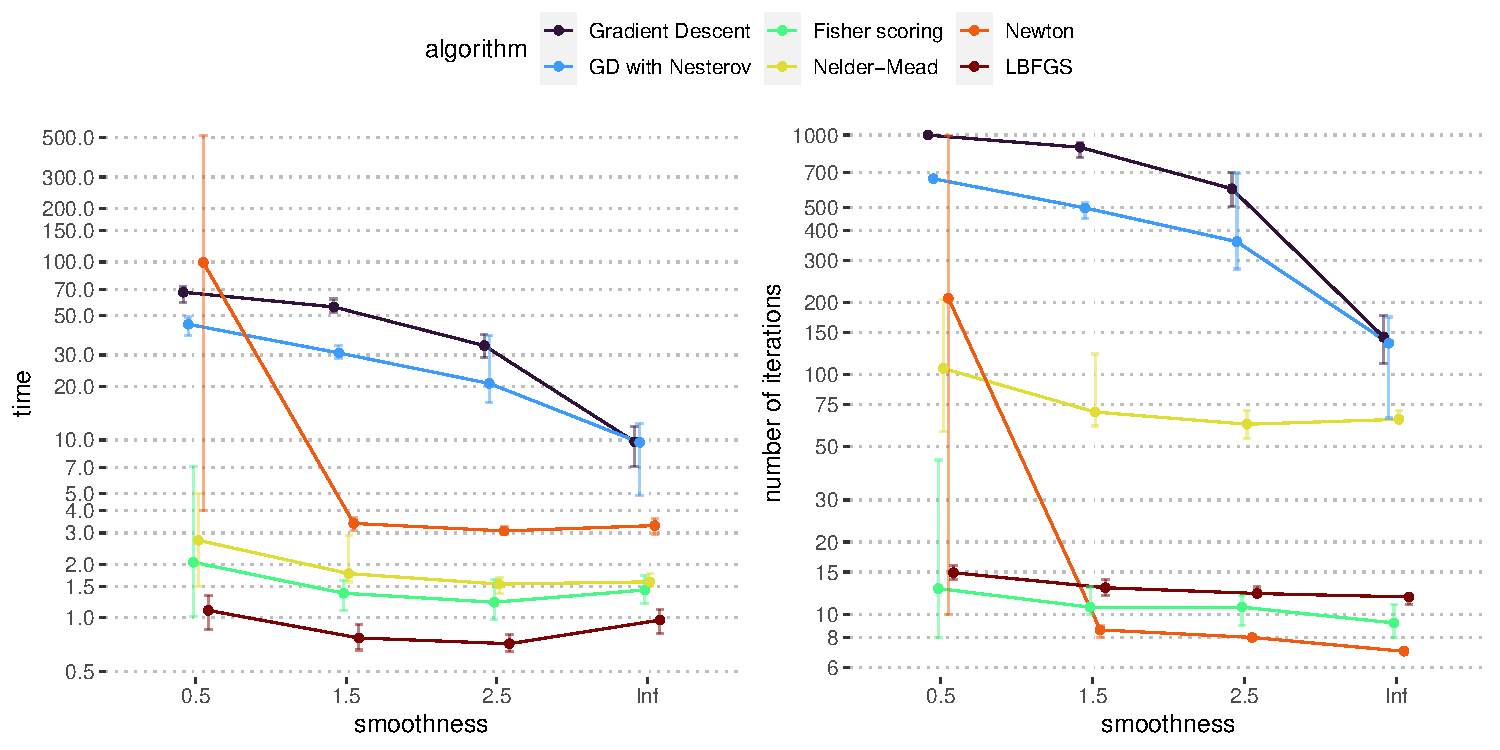
\includegraphics[width=.9\textwidth]{Borehole_comparison_0426} %<< no file extension
  %%         --- .5\textwidth stands for 50% of text width
  \caption[Times of Borehole function: line graphs with range bars]%<<-- Legend for the list of figures at the beginning of you thesis
  {Comparison of different methods using mis-specified GP models on data from Borehole function, default starting values, 10 repetitions. Y-axes are in $\log 10$ scale.}% legend displayed below the graph.
  \label{fig:plotset}
\end{figure}

\subsection{Piston function}

The 7-dimensional Piston function, which models the circular motion of a piston within a cylinder, is sampled with 1000 uniformly distributed points, and the results are displayed in Figure 3.18. The convergence check shows that when $\nu=0.5$, Newton's method fails to converge in 2 (of 10) repetitions. 

\begin{figure}[hbt!]%--- Picture 'H'ere, 'B'ottom or 'T'op; '!' 
  \centering
  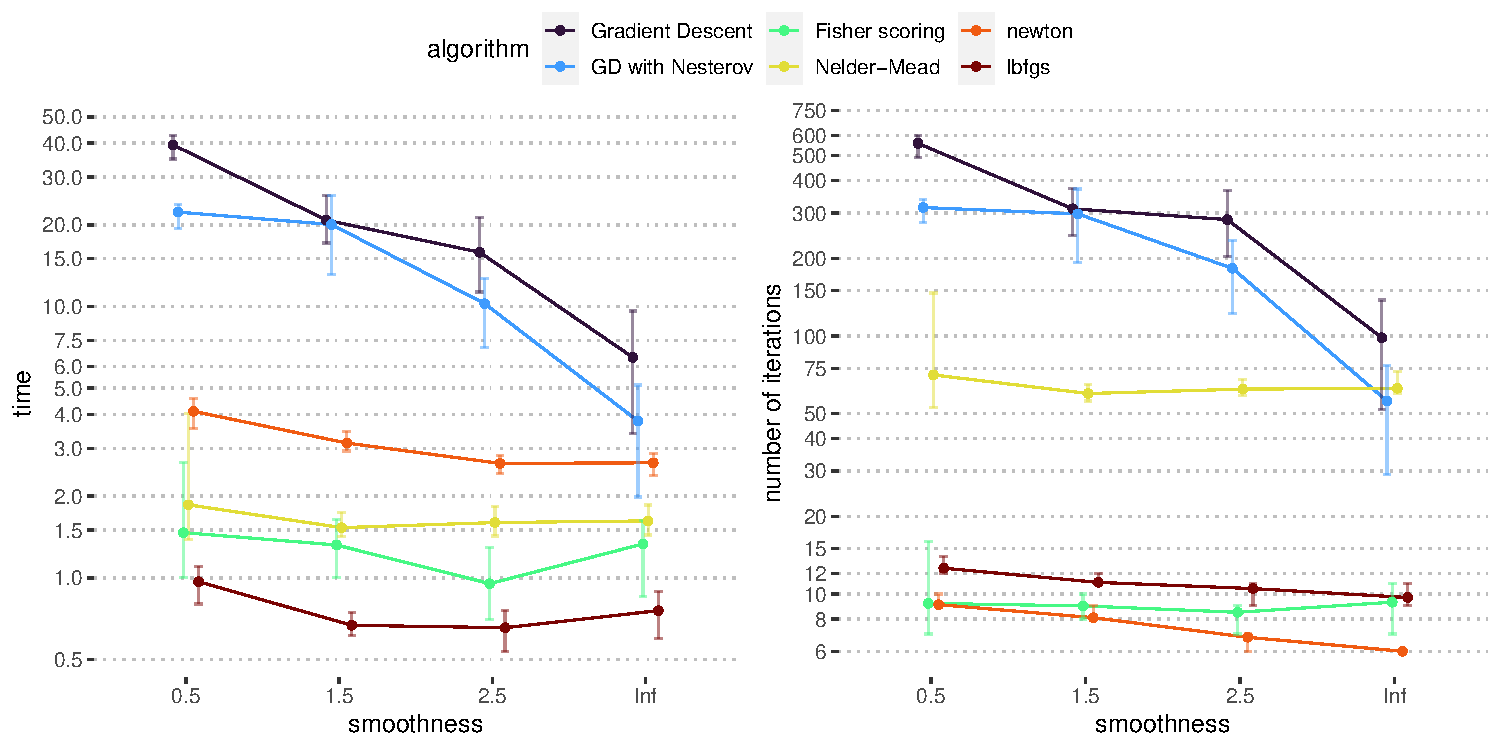
\includegraphics[width=.9\textwidth]{Piston_comparison_0426} %<< no file extension
  %%         --- .5\textwidth stands for 50% of text width
  \caption[Times of Piston function: line graphs with range bars]%<<-- Legend for the list of figures at the beginning of you thesis
  {Comparison of different methods using mis-specified GP models on data from Piston function, default starting values, 10 repetitions. Y-axes are in $\log 10$ scale.}% legend displayed below the graph.
  \label{fig:plotset}
\end{figure}

\subsection{Large scale optimization}

We want to explore the performance of optimization methods on the large scale of deterministic functions. We generate random samples of 20000 points and fit GP-Mat\'ern models with Vecchia approximation. Again, we perform the convergence check, but with stricter relative tolerance of 0.0001, since the original tolerance would not be precise enough due to the large log-likelihood values of this sample size. 

The results of Branin, Borehole, and Piston functions are displayed in Figures 3.19, 3.20 and 3.21. Among the six optimization methods, LBFGS consistently shows excellent performance of optimization for all of the three deterministic functions. 


\begin{figure}[hbt!]%--- Picture 'H'ere, 'B'ottom or 'T'op; '!' Try to
                    %impose your will to LaTeX
  \centering
  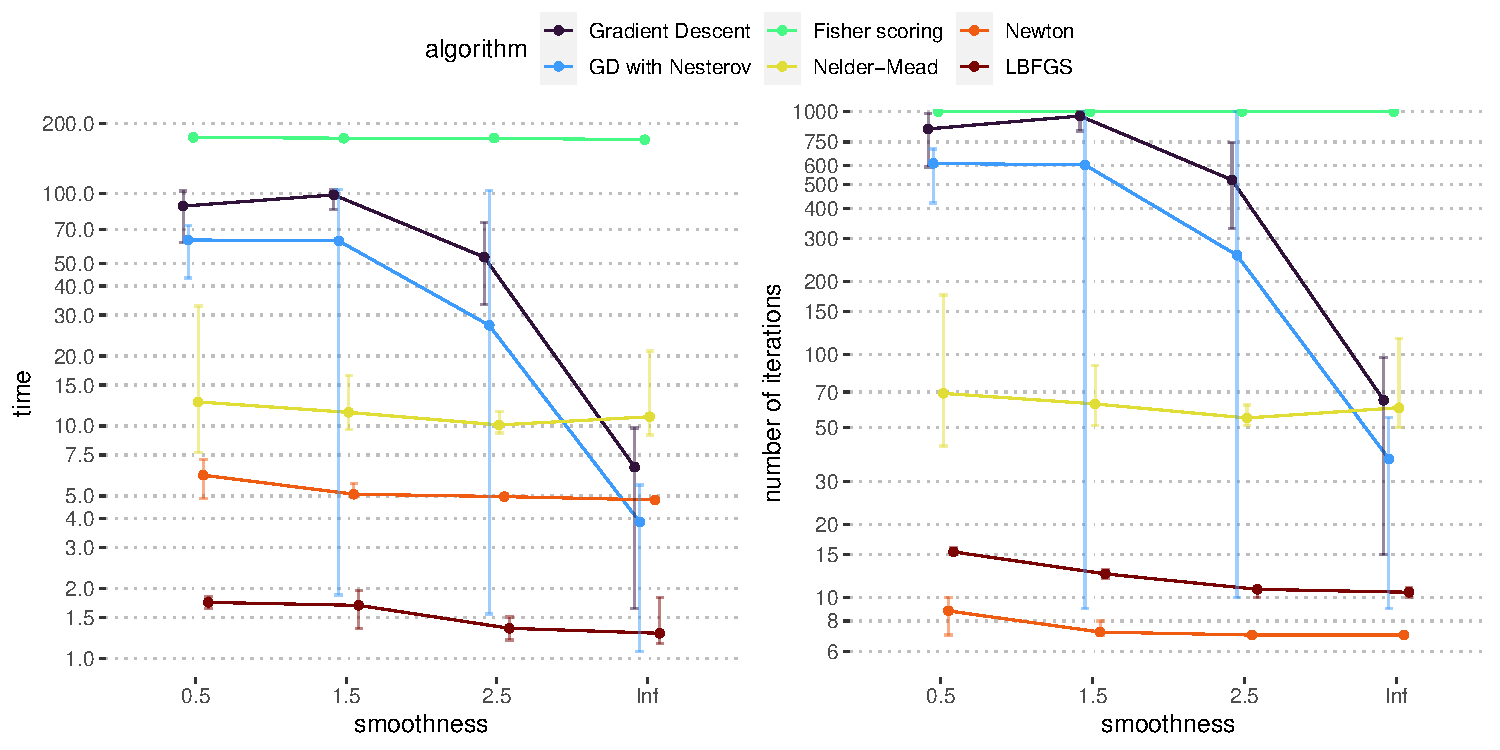
\includegraphics[width=.9\textwidth]{Branin_20000} %<< no file extension
  %%         --- .5\textwidth stands for 50% of text width
  \caption[Times of Branin of 20000 points: line graphs with range bars]%<<-- Legend for the list of figures at the beginning of you thesis
  {Comparison of different methods using GP models on 20000 points data from Branin function, default starting values, 10 repetitions. Y-axes are in $\log 10$ scale.}% legend displayed below the graph.
  \label{fig:plotset}
\end{figure}

\begin{figure}[hbt!]%--- Picture 'H'ere, 'B'ottom or 'T'op; '!' Try to
                    %impose your will to LaTeX
  \centering
  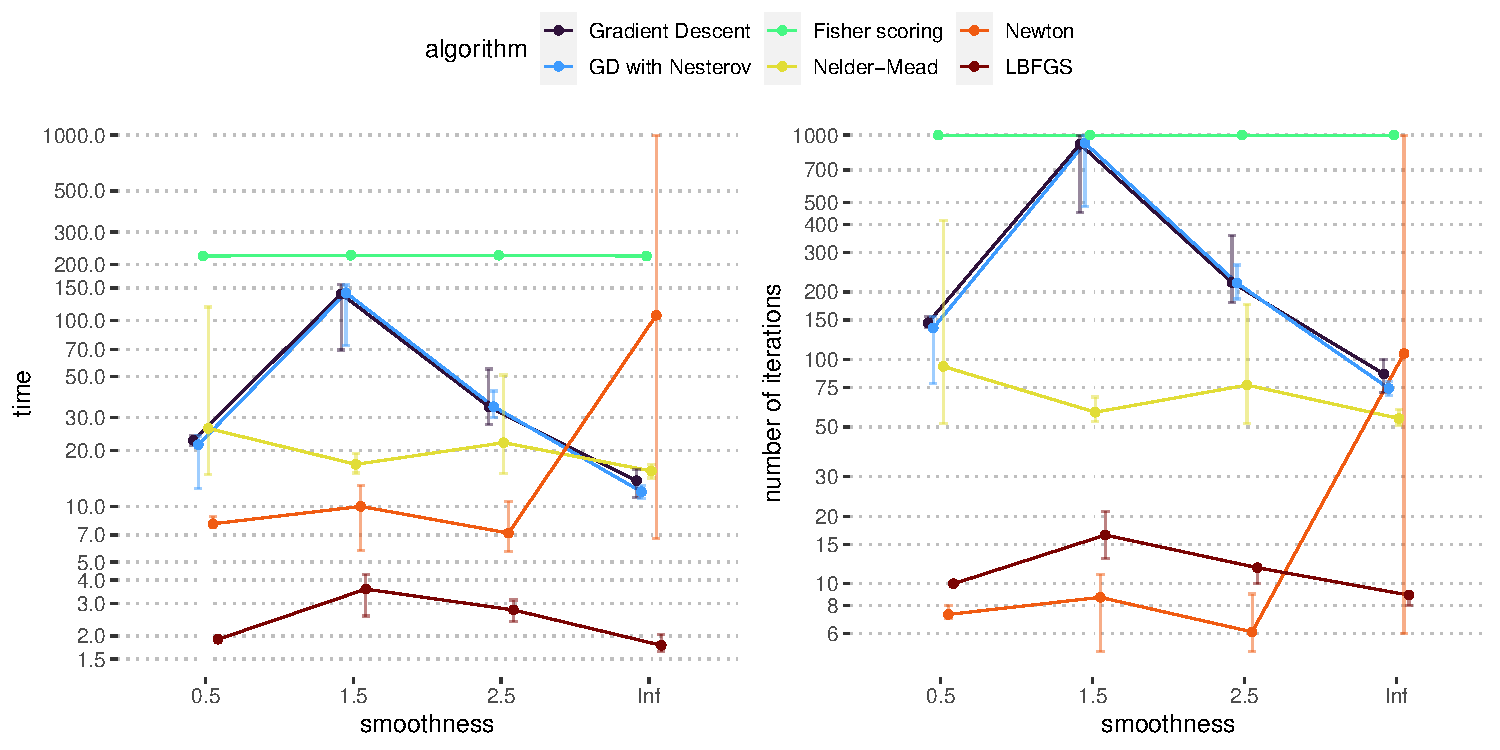
\includegraphics[width=.9\textwidth]{Borehole_20000} %<< no file extension
  %%         --- .5\textwidth stands for 50% of text width
  \caption[Times of Borehole of 20000 points: line graphs with range bars]%<<-- Legend for the list of figures at the beginning of you thesis
  {Comparison of different methods using GP models on 20000 points data from Borehole function, default starting values, 10 repetitions. Y-axes are in $\log 10$ scale.}% legend displayed below the graph.
  \label{fig:plotset}
\end{figure}

\begin{figure}[hbt!]%--- Picture 'H'ere, 'B'ottom or 'T'op; '!' Try to
                    %impose your will to LaTeX
  \centering
  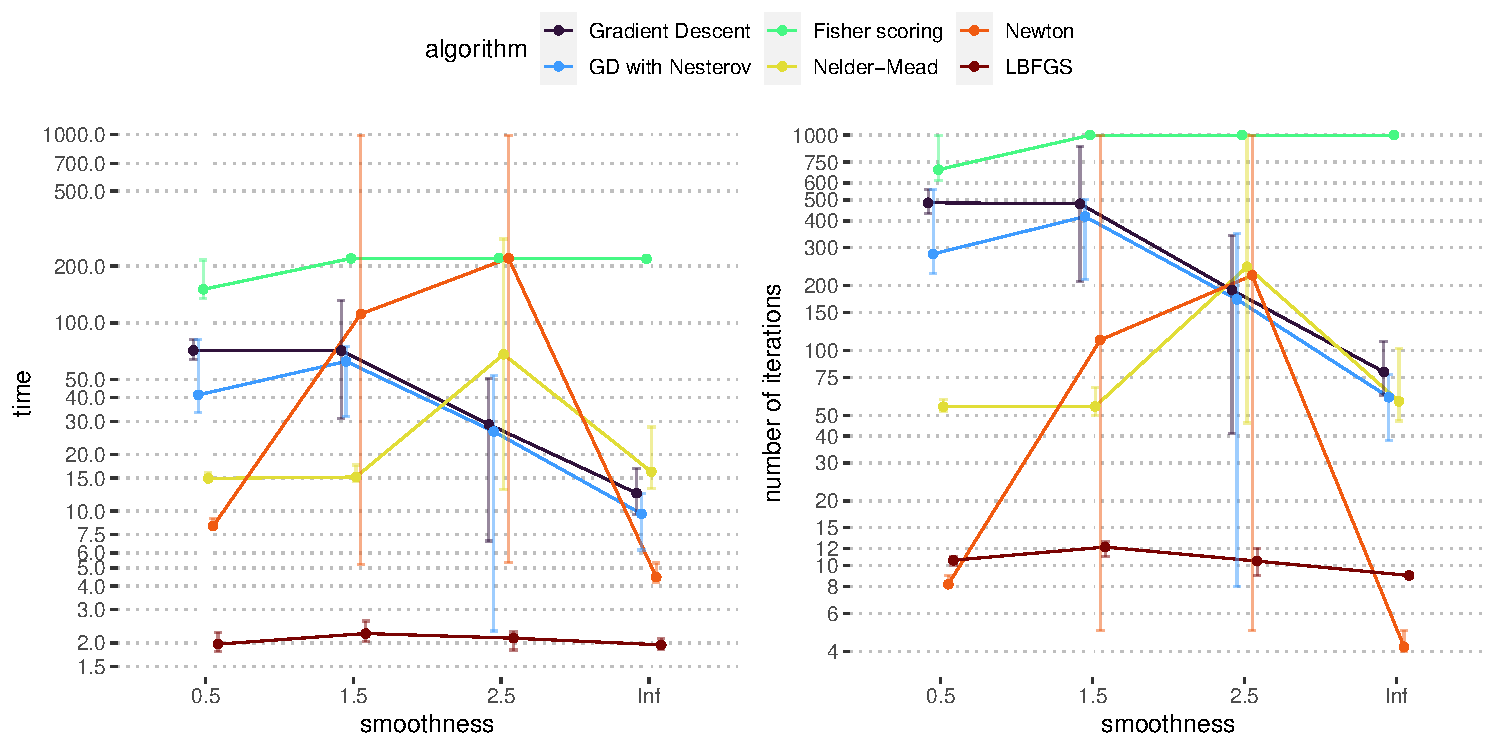
\includegraphics[width=.9\textwidth]{Piston_20000} %<< no file extension
  %%         --- .5\textwidth stands for 50% of text width
  \caption[Times of Piston of 20000 points: line graphs with range bars]%<<-- Legend for the list of figures at the beginning of you thesis
  {Comparison of different methods using GP models on 20000 points data from Piston function, default starting values, 10 repetitions. Y-axes are in $\log 10$ scale.}% legend displayed below the graph.
  \label{fig:plotset}
\end{figure}

The convergence problems of Branin large data experiment are:


\begin{itemize}
    \item With any smoothness, Fisher-scoring fails to converge within prescribed 1000 steps in any repetition.
    \item When $\nu = 1.5$, GD with Nesterov accelerator fails in 5 (of 10) repetitions.
\end{itemize}

For experiment of large data from Borehole function, the convergence check shows that:

\begin{itemize}
    \item With any smoothness, Fisher-scoring fails to converge within prescribed 1000 steps in any repetition of all smoothness settings.
    \item When $\nu = 1.5$, Newton fails in 2 (of 10) repetitions.
    \item When $\nu = 2.5$, Newton fails in 8 (of 10) repetitions.
    \item When $\nu = \inf$, Newton fails in 1 (of 10) repetition.
\end{itemize}

For experiment of large data from Piston function, the convergence check shows that:

\begin{itemize}
    \item When $\nu=0.5$, Fisher-scoring fails in 5 (of 10) repetitions.
    \item When $\nu=1.5$, 2.5, or $\infty$, Fisher-scoring fails to converge within prescribed 1000 iterations in all repetitions.
    \item When $\nu = 1.5$, Newton fails in 8 (of 10) repetitions.
    \item When $\nu = 2.5$, Newton fails in 10 (of 10) repetitions, Nelder-Mead fails in 2 (of 10) repetitions.
\end{itemize}





%%% Local Variables: 
%%% mode: latex
%%% TeX-master: "MasterThesisSfS"
%%% End: 
